% Author: Simon-Pierre Boucher — contact@spboucher.ai
%
% ═══════════════════════════════════════════════════════════════════════
% 5. RESULTS
% ═══════════════════════════════════════════════════════════════════════
\section{Estimation Results}
\label{sec:results}

\subsection{OLS Baseline, State Fixed Effects, and ZIP3 Fixed Effects}
\label{sec:ols_fe}

\subsubsection{Standardized Baseline Specification}

Table~\ref{tab:ols_results} presents the OLS results with standardized continuous regressors. The model achieves $R^2 = 0.634$ with RMSE $= 0.489$ in log-price units. The $F$-statistic of 18,712.5 strongly rejects the null of jointly zero slope coefficients.

\begin{table}[H]
\centering
\caption{OLS Hedonic Regression Results (Dep.\ Var.: $\ln(\text{Listing Price})$)}
\label{tab:ols_results}
\begin{threeparttable}
\small
\begin{tabular}{lrrl}
\toprule
Variable & Coefficient & Std.\ Error & \\
\midrule
\multicolumn{4}{l}{\textit{Panel A: Structural Attributes (standardized)}} \\
$\ln$(Living Area)$^\dagger$ & 0.3119 & 0.0035 & *** \\
Bedrooms$^\dagger$ & $-$0.0675 & 0.0023 & *** \\
Bathrooms$^\dagger$ & 0.2359 & 0.0026 & *** \\
Age$^\dagger$ & $-$0.0418 & 0.0139 & ** \\
Age$^{2\dagger}$ & 0.0507 & 0.0019 & *** \\
Stories$^\dagger$ & 0.0004 & 0.0003 & \\
Bath/Bed Ratio$^\dagger$ & $-$0.0208 & 0.0021 & *** \\
\midrule
\multicolumn{4}{l}{\textit{Panel B: Lot and Amenities}} \\
$\ln$(Lot Size)$^\dagger$ & 0.0697 & 0.0010 & *** \\
Pool & 0.0286 & 0.0026 & *** \\
Spa & 0.0327 & 0.0027 & *** \\
Basement & $-$0.0424 & 0.0023 & *** \\
Garage & 0.1094 & 0.0015 & *** \\
Waterfront & $-$0.1349 & 0.0325 & *** \\
Central Air & 0.0693 & 0.0014 & *** \\
Hardwood Floors & 0.1246 & 0.0014 & *** \\
Luxury Score$^\dagger$ & 0.0443 & 0.0018 & *** \\
\midrule
\multicolumn{4}{l}{\textit{Panel C: Neighborhood (standardized)}} \\
Walk Score$^\dagger$ & $-$0.0109 & 0.0012 & *** \\
Bike Score$^\dagger$ & 0.0717 & 0.0010 & *** \\
Transit Score$^\dagger$ & 0.0524 & 0.0008 & *** \\
Avg.\ School Rating$^\dagger$ & $-$0.0491 & 0.0007 & *** \\
Property Tax Rate$^\dagger$ & $-$0.0292 & 0.0008 & *** \\
\midrule
\multicolumn{4}{l}{\textit{Panel D: Market Status}} \\
Condominium & $-$0.0370 & 0.0037 & *** \\
HOA Member & $-$0.1077 & 0.0024 & *** \\
$\ln$(HOA Fees + 1)$^\dagger$ & 0.0439 & 0.0014 & *** \\
New Construction & 0.1035 & 0.0029 & *** \\
Foreclosure & $-$0.4064 & 0.0098 & *** \\
\midrule
\multicolumn{4}{l}{\textit{Panel E: Interactions (standardized)}} \\
$\ln$(sqft) $\times$ Age$^\dagger$ & $-$0.1100 & 0.0140 & *** \\
Pool $\times$ South & 0.0081 & 0.0012 & *** \\
Waterfront $\times$ $\ln$(sqft)$^\dagger$ & 0.1371 & 0.0092 & *** \\
Basement $\times$ North & $-$0.0255 & 0.0012 & *** \\
Condo $\times$ Walk Score$^\dagger$ & 0.0816 & 0.0013 & *** \\
Age $\times$ Luxury$^\dagger$ & 0.0440 & 0.0015 & *** \\
\midrule
\multicolumn{4}{l}{\textit{Panel F: Regional Dummies (ref: Midwest)}} \\
Northeast & 0.4869 & 0.0030 & *** \\
South & 0.0220 & 0.0028 & *** \\
West & 0.4008 & 0.0031 & *** \\
\midrule
$R^2$ & 0.6343 & & \\
Adj.\ $R^2$ & 0.6342 & & \\
RMSE & 0.4887 & & \\
$F$-statistic & 18,712.5 & & \\
$N$ & 788,842 & & \\
\bottomrule
\end{tabular}
\begin{tablenotes}
\small
\item \textit{Notes:} HC3 heteroskedasticity-robust standard errors. $^\dagger$Variables standardized (zero mean, unit variance) before estimation; coefficients represent effects of a one-standard-deviation increase. Binary variables not standardized; percentage effects computed as $100 \times (e^\beta - 1)$. Categorical controls (roof: 6, construction: 8, foundation: 7 dummies) included but not shown. Significance: *** $p<0.001$, ** $p<0.01$, * $p<0.05$.
\end{tablenotes}
\end{threeparttable}
\end{table}

\subsubsection{Unstandardized Specification for Economic Interpretation}

Table~\ref{tab:ols_unstd} reports key coefficients from the unstandardized specification, which permits direct economic interpretation. The $R^2$ is identical (0.634); only the coefficient magnitudes and interpretations differ.

\begin{table}[H]
\centering
\caption{Unstandardized OLS: Key Coefficients in Natural Units}
\label{tab:ols_unstd}
\begin{threeparttable}
\small
\begin{tabular}{lrrrl}
\toprule
Variable & Coefficient & Std.\ Error & Interpretation & \\
\midrule
Constant & 7.7316 & 0.0495 & & *** \\
$\ln$(Living Area) & 0.6281 & 0.0070 & Elasticity: 0.63 & *** \\
Bedrooms & $-$0.0620 & 0.0022 & $-$6.0\% per additional bedroom & *** \\
Bathrooms & 0.2035 & 0.0023 & +22.6\% per additional bathroom & *** \\
Age (years) & $-$0.0013 & 0.0004 & $-$0.13\% per year & ** \\
Age$^2$ ($\times 10^{-5}$) & 1.2 & 0.05 & Positive quadratic (vintage) & *** \\
$\ln$(Lot Size) & 0.0182 & 0.0003 & Elasticity: 0.02 & *** \\
Walk Score (per point) & $-$0.0004 & 0.0000 & $-$0.04\% per point & *** \\
Bike Score (per point) & 0.0040 & 0.0001 & +0.40\% per point & *** \\
Transit Score (per point) & 0.0029 & 0.0000 & +0.29\% per point & *** \\
Avg.\ School Rating (per point) & $-$0.0544 & 0.0008 & $-$5.3\% per rating point & *** \\
Property Tax Rate (per ppt) & $-$0.0553 & 0.0015 & $-$5.4\% per ppt & *** \\
Luxury Score (per unit) & 0.0344 & 0.0014 & +3.5\% per unit & *** \\
\bottomrule
\end{tabular}
\begin{tablenotes}
\small
\item \textit{Notes:} Same sample and specification as Table~\ref{tab:ols_results}, but continuous variables enter in natural units. $N = 788{,}842$. HC3 standard errors.
\end{tablenotes}
\end{threeparttable}
\end{table}

The elasticity of listing price with respect to living area is 0.63: a 10\% increase in square footage is associated with a 6.3\% higher listing price. This is below unity, consistent with diminishing marginal returns to space. Each additional bathroom is associated with a 22.6\% higher listing price, while each additional bedroom---conditional on total area---is associated with a 6.0\% \textit{lower} price, reflecting the well-documented tradeoff between room count and room size \citep{sirmans2005composition}.

\subsubsection{Counterintuitive Coefficient Signs}

Several coefficients warrant discussion.

\textbf{Negative waterfront coefficient ($-0.135$, standardized).} The standalone waterfront effect is evaluated at the mean of the standardized interaction term $\text{waterfront} \times \ln(\text{sqft})$. Because the interaction is strongly positive ($+0.137$), the net waterfront effect becomes positive for larger properties. This artifact of the interacted specification does not imply that waterfront reduces price on average.

\textbf{Negative school rating ($-0.054$ per rating point, unstandardized).} This likely reflects confounding with property tax rates and regional effects. In higher-tax jurisdictions, school quality is partially capitalized through the tax rate, which enters separately. Conditional on tax rate, region, and other controls, the residual school rating variation may capture unobserved factors that correlate negatively with prices. The boundary-discontinuity literature, which isolates school quality from neighborhood composition, consistently finds positive valuations \citep{black1999better, bayer2007unified}; the divergence illustrates why cross-sectional partial coefficients on school quality should not be interpreted structurally.

\textbf{Negative Walk Score ($-0.0004$ per point, unstandardized).} Walk Score is highly correlated with Bike Score ($r \approx 0.56$) and Transit Score ($r \approx 0.62$). In the presence of all three accessibility measures, the Walk Score coefficient may reflect residual urban density effects---after controlling for biking and transit access, the remaining variation in walkability may capture denser, smaller-lot neighborhoods. A walkability premium is well documented when accessibility enters alone \citep{pivo2011walkability}; with three collinear accessibility scores, the premium is split across coefficients and cannot be attributed variable-by-variable.

\textbf{Negative basement ($-0.042$).} Basements are predominantly found in older properties in colder regions. Conditional on age, region, and size, the basement indicator may proxy for older construction quality or layout features valued less in modern markets.

\textbf{Negative HOA membership ($-0.108$).} HOA properties include condominiums and planned communities that may have lower lot sizes and more restrictions. The negative sign is conditional on the separate log HOA fee variable ($+0.044$), suggesting that the HOA membership dummy captures the property-type effect while fees capture the service-quality gradient.

These counterintuitive signs are common in hedonic regressions with many correlated controls and do not necessarily indicate misspecification, though they do limit the attributable economic interpretation of individual coefficients.

\subsubsection{Progressive Geographic Fixed Effects}
\label{sec:progressive_fe}

Table~\ref{tab:fe_comparison} documents how explanatory power increases with geographic granularity. Adding 50 state fixed effects increases the in-sample $R^2$ from 0.634 to 0.681. Replacing state dummies with 886 ZIP3 fixed effects further increases $R^2$ to 0.729 (in-sample) and out-of-sample $R^2$ to 0.725.

\begin{table}[H]
\centering
\caption{OLS $R^2$ Under Progressively Finer Geographic Controls}
\label{tab:fe_comparison}
\begin{threeparttable}
\begin{tabular}{lrrrr}
\toprule
Specification & Geographic FE & $N_{\text{FE}}$ & In-sample $R^2$ & Out-of-sample $R^2$ \\
\midrule
Baseline (4 regions) & Census Region & 3 & 0.634 & 0.630 \\
State FE & State & 50 & 0.681 & 0.678 \\
ZIP3 FE & 3-digit ZIP & 886 & 0.729 & 0.725 \\
\bottomrule
\end{tabular}
\begin{tablenotes}
\small
\item \textit{Notes:} Same 62 non-geographic regressors across all specifications; geographic FE replace the 3 regional dummies. Out-of-sample $R^2$ computed on a random 20\% holdout. ZIP3 codes cover 886 unique prefixes in the sample.
\end{tablenotes}
\end{threeparttable}
\end{table}

The progression from region to state to ZIP3 fixed effects yields $R^2$ gains of $+4.7$ pp and $+4.7$ pp, respectively. This 9.5 pp total gain from geographic granularity alone---achieved without any additional property-level information---underscores the importance of unobserved local factors in hedonic pricing. Notably, even ZIP3 fixed effects leave substantial residual variation unexplained: the gap between ZIP3 OLS ($R^2 = 0.725$) and XGBoost under random validation ($R^2 = 0.833$) suggests that non-linear attribute effects contribute an additional 10.8 pp of explained variation.

\subsubsection{OLS Diagnostics}

Figure~\ref{fig:diagnostics} presents diagnostic plots. The residual distribution exhibits excess kurtosis (5.55 vs.\ 3.0 for normality) and mild positive skewness (0.18), as confirmed by the Jarque-Bera test ($JB = 217{,}078$, $p < 0.001$). The heteroskedastic pattern visible in the residuals-versus-fitted plot motivates our use of HC3 standard errors.

\begin{figure}[H]
    \centering
    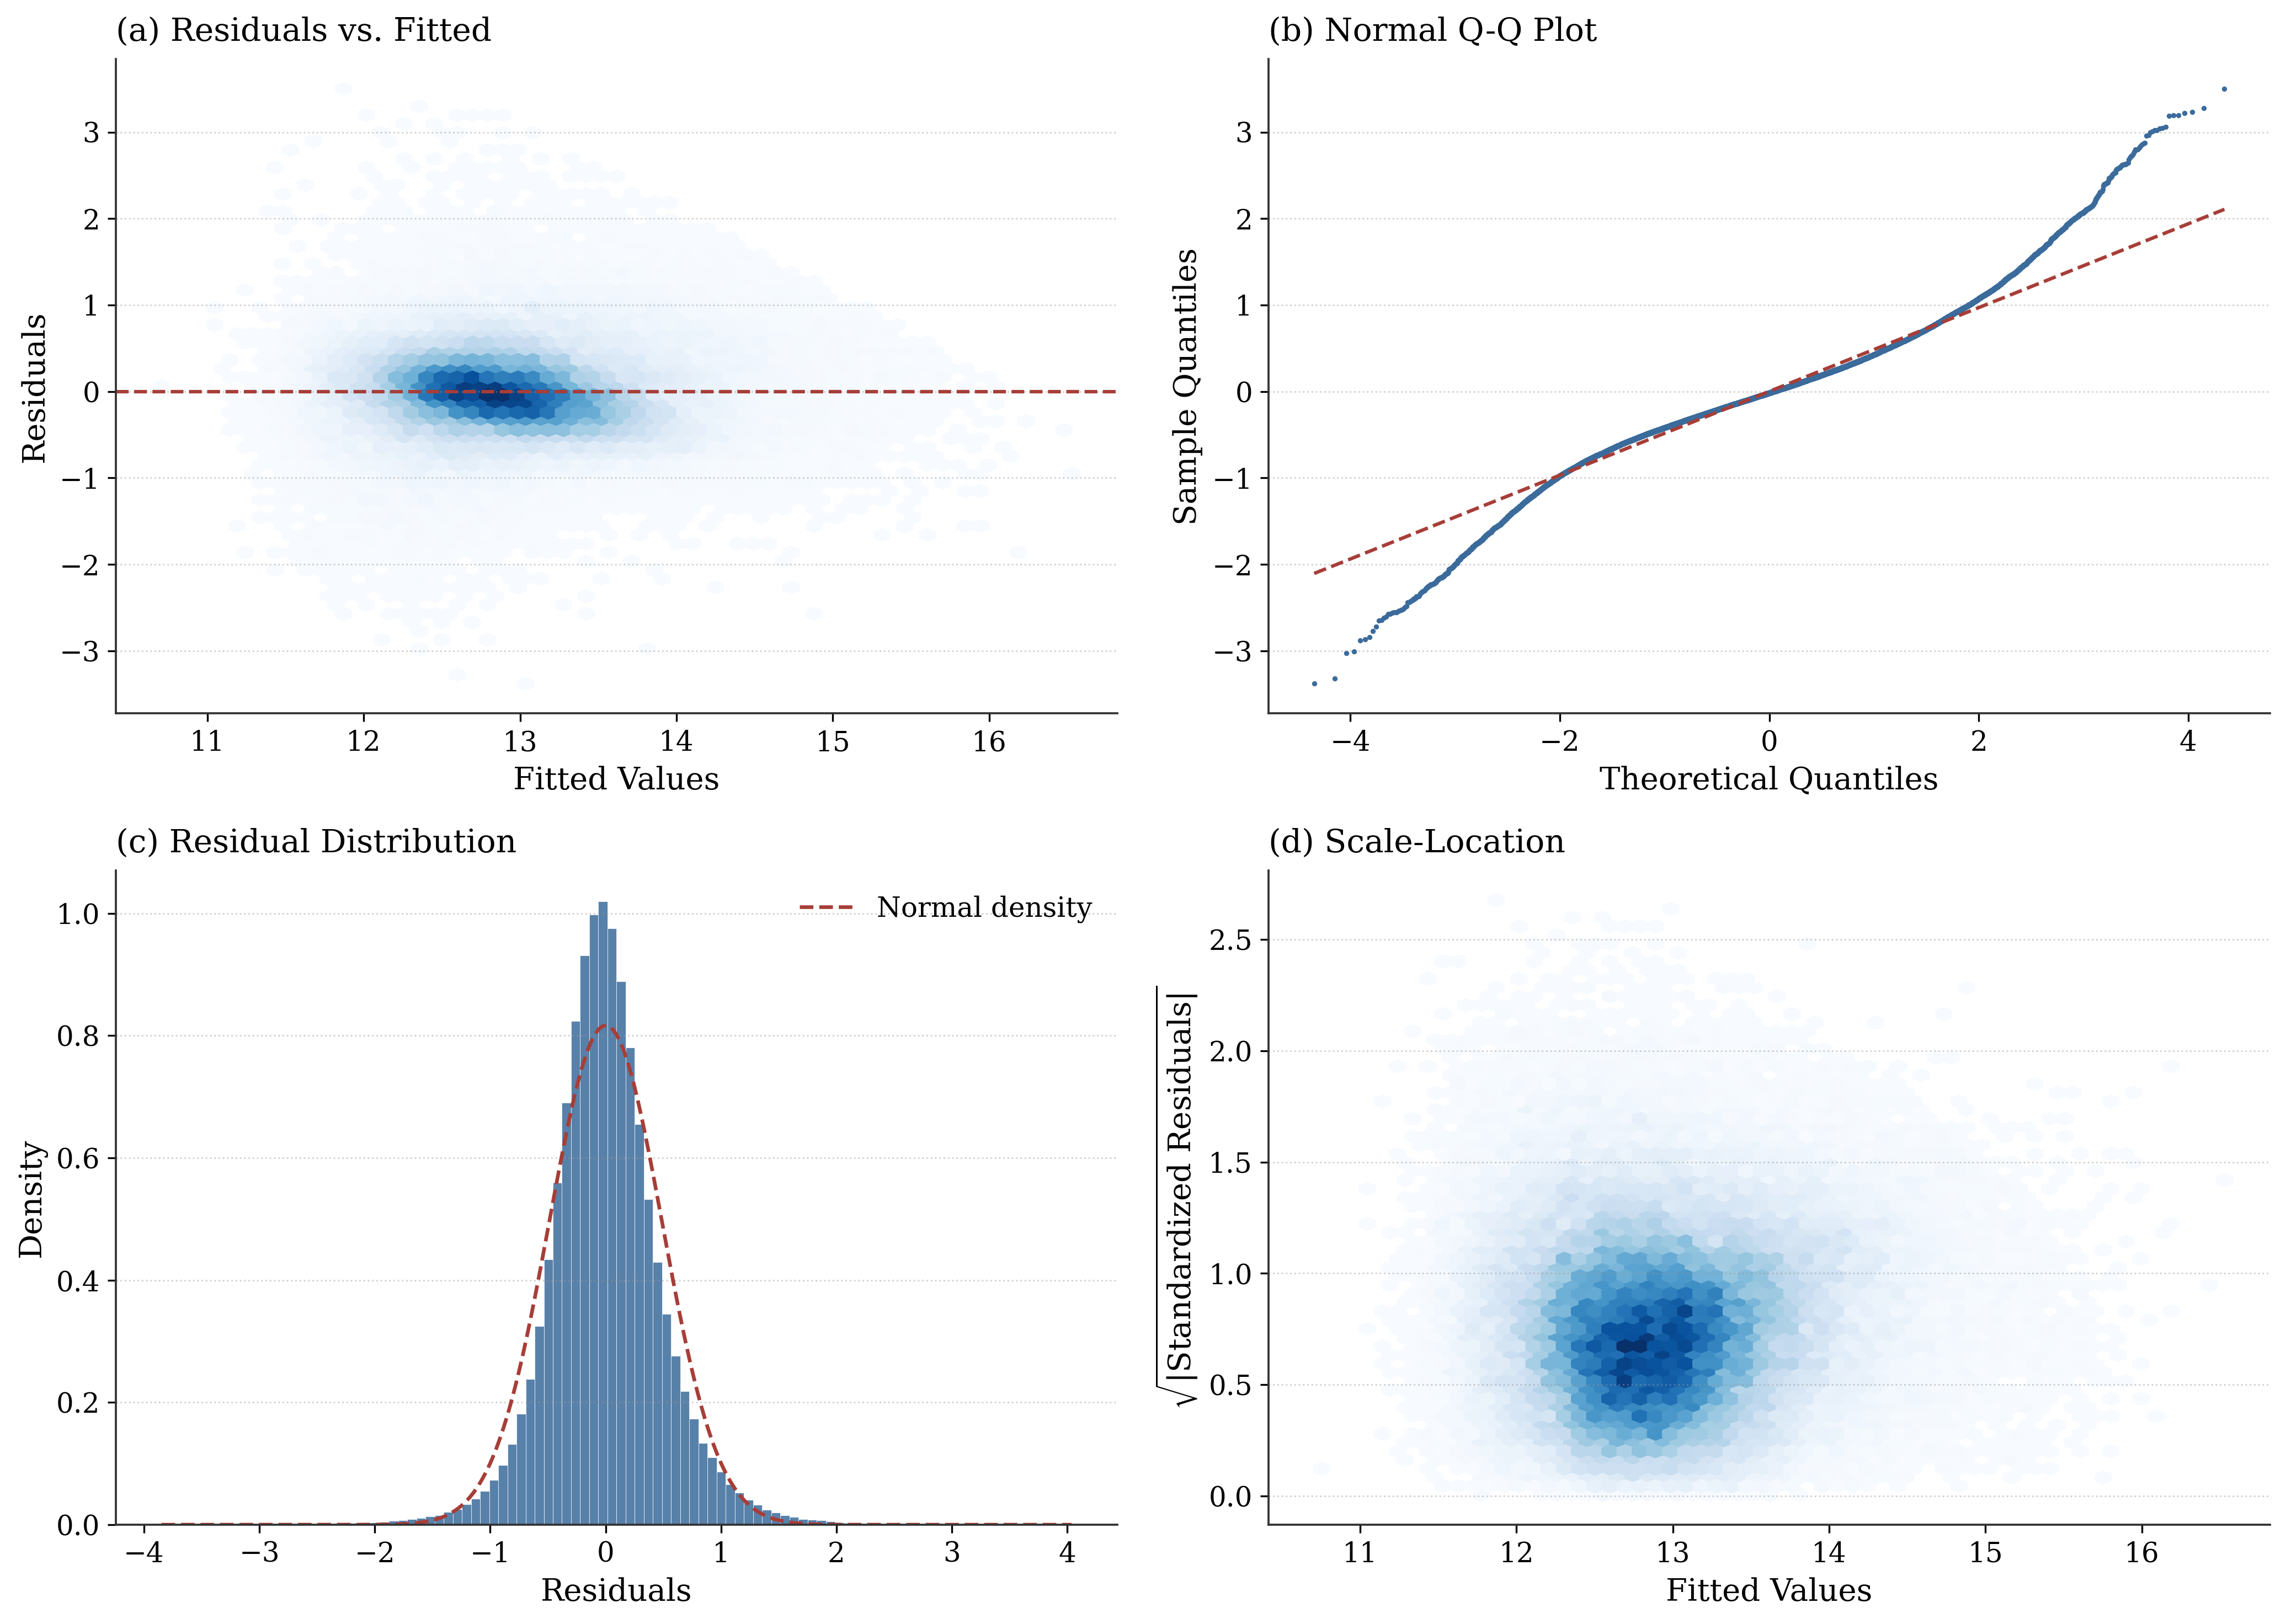
\includegraphics[width=\textwidth]{figures/fig2_ols_diagnostics.png}
    \caption{OLS Diagnostic Plots: (a) Residuals vs.\ Fitted; (b) Normal Q-Q Plot; (c) Residual Distribution; (d) Scale-Location}
    \label{fig:diagnostics}
\end{figure}


\subsection{Spatial Autocorrelation}
\label{sec:spatial_autocorrelation}

We compute Moran's $I$ on OLS residuals using a KNN spatial weight matrix ($k = 8$) on three independent random subsamples of 5,000 observations each. Table~\ref{tab:moran} reports the results.

\begin{table}[H]
\centering
\caption{Moran's $I$ on OLS Residuals: Subsample Stability}
\label{tab:moran}
\begin{threeparttable}
\begin{tabular}{lrrrl}
\toprule
Subsample & $I$ & $z$-statistic & $p$-value & \\
\midrule
Subsample 1 & 0.2742 & 41.8 & $<0.001$ & *** \\
Subsample 2 & 0.2839 & 43.5 & $<0.001$ & *** \\
Subsample 3 & 0.2652 & 40.5 & $<0.001$ & *** \\
\midrule
Mean & 0.2745 & & & \\
Std.\ Dev. & 0.0076 & & & \\
\bottomrule
\end{tabular}
\begin{tablenotes}
\small
\item \textit{Notes:} Row-standardized KNN weight matrix with $k = 8$. Each subsample draws 5,000 observations at random. All $z$-statistics strongly reject the null of no spatial autocorrelation. The low standard deviation (0.008) across subsamples indicates that the diagnostic is highly stable.
\end{tablenotes}
\end{threeparttable}
\end{table}

The mean Moran's $I = 0.2745$ (std $= 0.0076$) across three subsamples confirms \textbf{strong, stable positive spatial autocorrelation} in the OLS residuals. This implies that our regional controls (four Census regions) are insufficient to absorb local price variation. OLS standard errors may understate true uncertainty, and coefficient estimates may be biased if the spatial structure correlates with included regressors. The stability across subsamples (CV $= 2.8\%$) indicates that this is not a sampling artifact but a structural feature of the data. Addressing spatial dependence through spatial econometric models is an important direction for future work; our OLS and quantile regression results should be interpreted with this caveat.


\subsection{Quantile Regression and Inter-Quantile Tests}
\label{sec:qr_results}

\subsubsection{Coefficient Estimates Across Quantiles}

Table~\ref{tab:qr_results} presents quantile regression coefficients at the five estimated quantiles.

\begin{table}[H]
\centering
\caption{Quantile Regression Coefficients at Selected Quantiles}
\label{tab:qr_results}
\begin{threeparttable}
\small
\begin{tabular}{lrrrrrr}
\toprule
Variable & $\tau=0.10$ & $\tau=0.25$ & $\tau=0.50$ & $\tau=0.75$ & $\tau=0.90$ & OLS \\
\midrule
$\ln$(Living Area) & 0.358*** & 0.313*** & 0.275*** & 0.237*** & 0.251*** & 0.312*** \\
Bedrooms & $-$0.085*** & $-$0.076*** & $-$0.064*** & $-$0.037*** & $-$0.034*** & $-$0.068*** \\
Bathrooms & 0.157*** & 0.195*** & 0.234*** & 0.259*** & 0.259*** & 0.236*** \\
Age & $-$0.430*** & $-$0.201*** & $-$0.066** & $-$0.007 & $-$0.026 & $-$0.042** \\
$\ln$(Lot Size) & 0.045*** & 0.051*** & 0.061*** & 0.070*** & 0.086*** & 0.070*** \\
Pool & 0.008 & 0.008 & 0.019*** & 0.061*** & 0.094*** & 0.029*** \\
Garage & 0.205*** & 0.146*** & 0.102*** & 0.061*** & 0.020*** & 0.109*** \\
Luxury Score & 0.018*** & 0.038*** & 0.054*** & 0.068*** & 0.072*** & 0.044*** \\
Foreclosure & $-$0.494*** & $-$0.473*** & $-$0.379*** & $-$0.327*** & $-$0.338*** & $-$0.406*** \\
Northeast & 0.339*** & 0.395*** & 0.471*** & 0.553*** & 0.603*** & 0.487*** \\
West & 0.365*** & 0.372*** & 0.376*** & 0.399*** & 0.450*** & 0.401*** \\
\bottomrule
\end{tabular}
\begin{tablenotes}
\small
\item \textit{Notes:} Estimated on a random subsample of 150,000 observations. Continuous variables standardized. Full set of 62 regressors included; selected coefficients shown. Significance: *** $p<0.001$, ** $p<0.01$, * $p<0.05$. Coefficients reflect one-standard-deviation effects for continuous variables.
\end{tablenotes}
\end{threeparttable}
\end{table}

\begin{figure}[H]
    \centering
    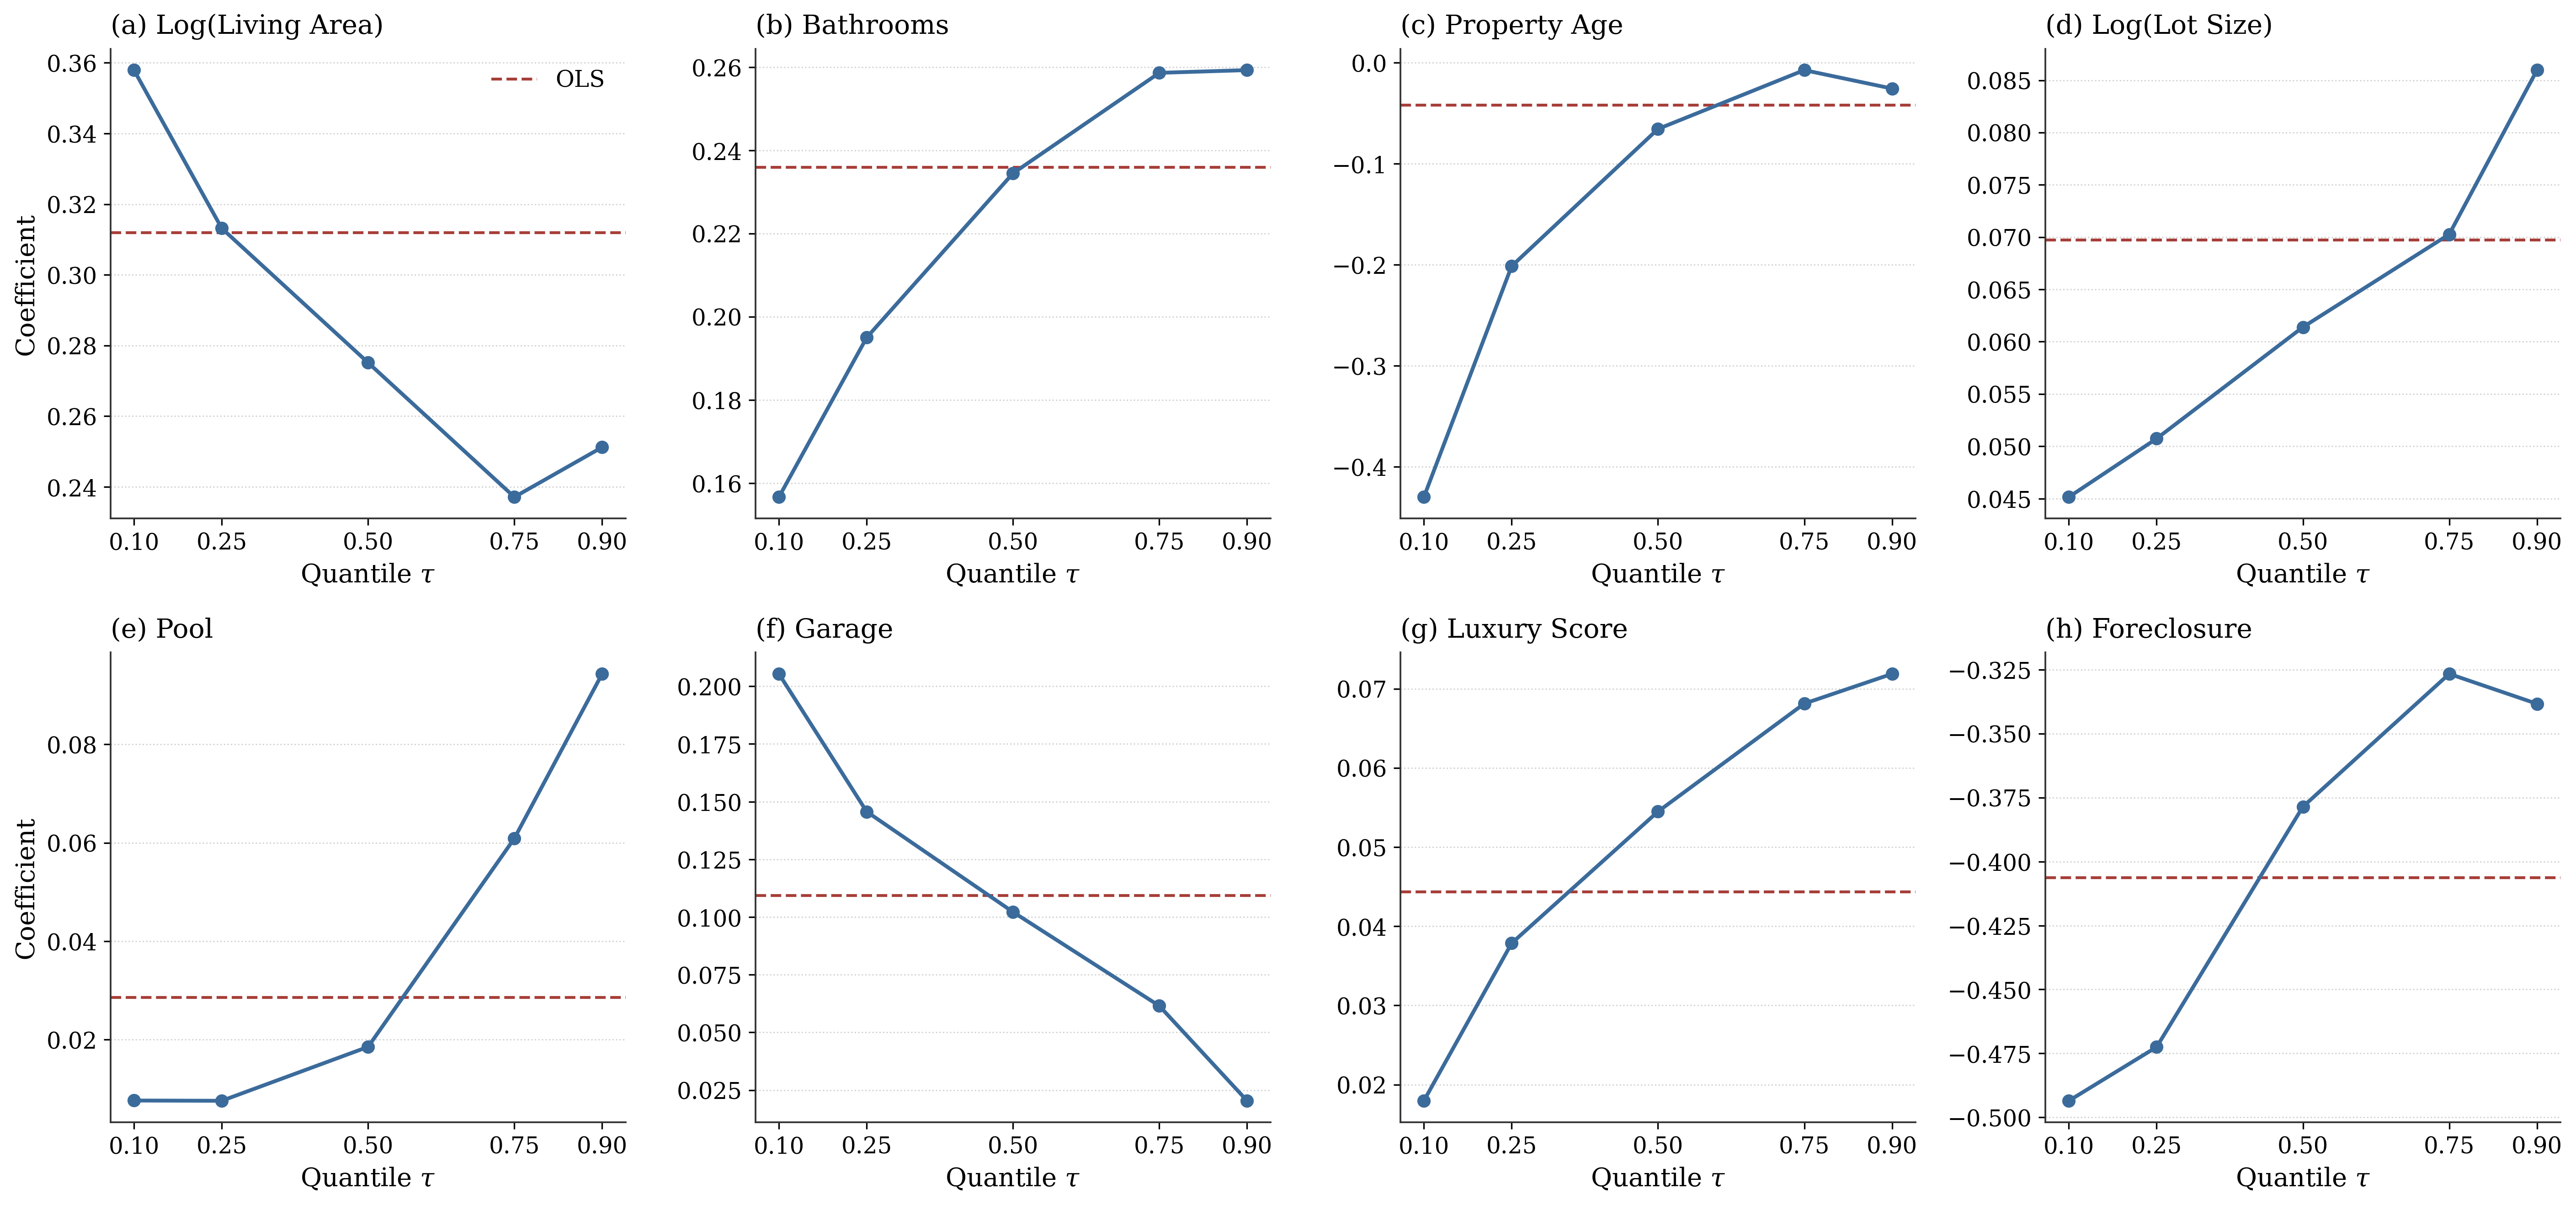
\includegraphics[width=\textwidth]{figures/fig3_quantile_coefficients.png}
    \caption{Quantile Regression Coefficients Across the Conditional Price Distribution. Red dashed lines indicate OLS estimates. Coefficients are on standardized variables.}
    \label{fig:qr_coefficients}
\end{figure}

Several economically interesting patterns emerge.

\textbf{Living area gradient declines at upper quantiles.} The standardized $\ln(\text{sqft})$ coefficient declines from 0.358 ($\tau = 0.10$) to 0.237 ($\tau = 0.75$), indicating that additional space is associated with proportionally larger listing-price differences at the lower end of the conditional distribution. At higher quantiles, other factors (luxury features, location) may dominate size.

\textbf{Bathroom gradient increases at upper quantiles.} In contrast, the bathroom gradient rises monotonically from 0.157 ($\tau = 0.10$) to 0.259 ($\tau = 0.90$), suggesting that bathroom count differentiates properties more strongly in the upper market.

\textbf{Age penalty concentrated at lower quantiles.} The age gradient is $-0.430$ at $\tau = 0.10$ but statistically insignificant at $\tau = 0.75$ and $\tau = 0.90$. Age-related depreciation appears to be primarily a phenomenon of lower-priced properties, possibly because higher-priced properties are better maintained or benefit from vintage appeal.

\textbf{Pool gradient emerges only above the median.} The pool coefficient is insignificant at $\tau = 0.10$ and $\tau = 0.25$ but rises to 0.094 at $\tau = 0.90$ ($\approx 9.9\%$ listing-price difference), consistent with pools being a luxury amenity.

\textbf{Garage gradient declines monotonically.} The garage coefficient drops from 0.205 ($\tau = 0.10$) to 0.020 ($\tau = 0.90$), reflecting that garage availability differentiates lower-priced properties much more than upper-priced ones where garages are nearly universal.

OLS averages across these heterogeneous gradients and can therefore misrepresent both the lower and upper segments of the market.

\subsubsection{Inter-Quantile Wald Tests ($\tau = 0.10$ vs.\ $\tau = 0.90$)}

Table~\ref{tab:iqr_tests} reports the inter-quantile Wald tests for equality of coefficients between the 10th and 90th percentiles.

\begin{table}[H]
\centering
\caption{Inter-Quantile Wald Tests: $\hat{\beta}(0.10) - \hat{\beta}(0.90)$}
\label{tab:iqr_tests}
\begin{threeparttable}
\small
\begin{tabular}{lrrrl}
\toprule
Variable & $\hat{\beta}(0.10) - \hat{\beta}(0.90)$ & $z$-statistic & $p$-value & \\
\midrule
Garage & $+$0.185 & 28.92 & $<0.001$ & *** \\
Northeast & $-$0.264 & $-$21.43 & $<0.001$ & *** \\
Bathrooms & $-$0.103 & $-$10.48 & $<0.001$ & *** \\
$\ln$(Living Area) & $+$0.107 & 9.52 & $<0.001$ & *** \\
$\ln$(Lot Size) & $-$0.041 & $-$9.49 & $<0.001$ & *** \\
Age & $-$0.405 & $-$7.89 & $<0.001$ & *** \\
Pool & $-$0.087 & $-$7.80 & $<0.001$ & *** \\
Luxury Score & $-$0.054 & $-$6.82 & $<0.001$ & *** \\
West & $-$0.086 & $-$6.26 & $<0.001$ & *** \\
Bedrooms & $-$0.051 & $-$5.95 & $<0.001$ & *** \\
Foreclosure & $-$0.155 & $-$4.18 & $<0.001$ & *** \\
\midrule
\multicolumn{5}{l}{\textit{Not significant ($p > 0.05$)}} \\
Waterfront & $+$0.222 & 1.86 & 0.063 & \\
Age$^2$ & $+$0.010 & 1.40 & 0.162 & \\
\bottomrule
\end{tabular}
\begin{tablenotes}
\small
\item \textit{Notes:} $z$-statistics computed from the joint covariance matrix of the $\tau = 0.10$ and $\tau = 0.90$ quantile regression estimates; both quantiles estimated on the same 150,000-observation subsample. Variables sorted by $|z|$. 11 of 13 tested variables show statistically significant differences at the 5\% level. *** $p<0.001$, ** $p<0.01$, * $p<0.05$.
\end{tablenotes}
\end{threeparttable}
\end{table}

The inter-quantile tests reject coefficient equality for 11 of 13 tested variables at the 5\% level. The largest inter-quantile difference is for garage ($+0.185$, $z = 28.92$), confirming that the garage listing-price gradient is dramatically larger for lower-priced properties. Bathrooms ($-0.103$, $z = -10.48$) and living area ($+0.107$, $z = 9.52$) also exhibit large, highly significant inter-quantile differences. The only two variables for which the null of equal coefficients cannot be rejected are age-squared ($z = 1.40$) and waterfront ($z = 1.86$, $p = 0.063$).

These formal tests confirm the visual patterns in Figure~\ref{fig:qr_coefficients}: the conditional distribution of listing prices is not merely shifted by housing attributes but is differentially stretched and compressed, with different attributes mattering more at different points in the distribution.


\subsection{Machine Learning Under Random Validation}
\label{sec:ml_random}

Table~\ref{tab:ml_comparison} summarizes out-of-sample performance under the random 80/20 split.

\begin{table}[H]
\centering
\caption{Out-of-Sample Predictive Performance: Random Validation}
\label{tab:ml_comparison}
\begin{threeparttable}
\small
\begin{tabular}{lrrrrrr}
\toprule
 & \multicolumn{3}{c}{Log-Price Scale} & \multicolumn{3}{c}{Dollar Scale} \\
\cmidrule(lr){2-4} \cmidrule(lr){5-7}
Model & $R^2$ & RMSE & MAE & MAPE (\%) & MdAPE (\%) & MAE (\$) \\
\midrule
OLS & 0.6301 & 0.4911 & 0.3619 & 39.8 & 27.2 & 240,941 \\
Ridge ($\alpha=1$) & 0.6301 & 0.4911 & 0.3619 & --- & --- & --- \\
Lasso ($\alpha=0.001$) & 0.6280 & 0.4925 & 0.3627 & --- & --- & --- \\
Elastic Net & 0.6145 & 0.5014 & 0.3681 & --- & --- & --- \\
OLS + State FE & 0.6775 & 0.4586 & --- & --- & --- & --- \\
OLS + ZIP3 FE & 0.7253 & --- & --- & --- & --- & --- \\
Random Forest & 0.7842 & 0.3751 & 0.2636 & 28.4 & 18.5 & 180,116 \\
LightGBM & 0.8088 & 0.3531 & 0.2519 & 26.9 & 18.2 & 169,495 \\
\textbf{XGBoost} & \textbf{0.8330} & \textbf{0.3300} & \textbf{0.2327} & \textbf{24.7} & \textbf{16.5} & \textbf{157,822} \\
\bottomrule
\end{tabular}
\begin{tablenotes}
\small
\item \textit{Notes:} Training: 631,073 (80\%). Test: 157,769 (20\%). Random split, seed 42. MAPE = mean absolute percentage error; MdAPE = median APE. Dollar metrics computed by exponentiating predicted log-prices. Ridge, Lasso, Elastic Net dollar metrics suppressed for brevity (similar to OLS). ZIP3 FE RMSE and dollar-scale metrics not computed for this specification.
\end{tablenotes}
\end{threeparttable}
\end{table}

XGBoost achieves the highest $R^2$ of 0.833 under random validation, representing a 20-percentage-point improvement over OLS. Regularized linear models (Ridge, Lasso, Elastic Net) offer no improvement over OLS, confirming that the parametric specification is not overfit---the predictive gap is driven by non-linearity and interaction effects, not overfitting. The ZIP3 FE model ($R^2 = 0.725$) closes roughly half the OLS-to-XGBoost gap, indicating that fine-grained geographic controls capture a substantial portion of the non-linearity that tree models exploit.

\begin{figure}[H]
    \centering
    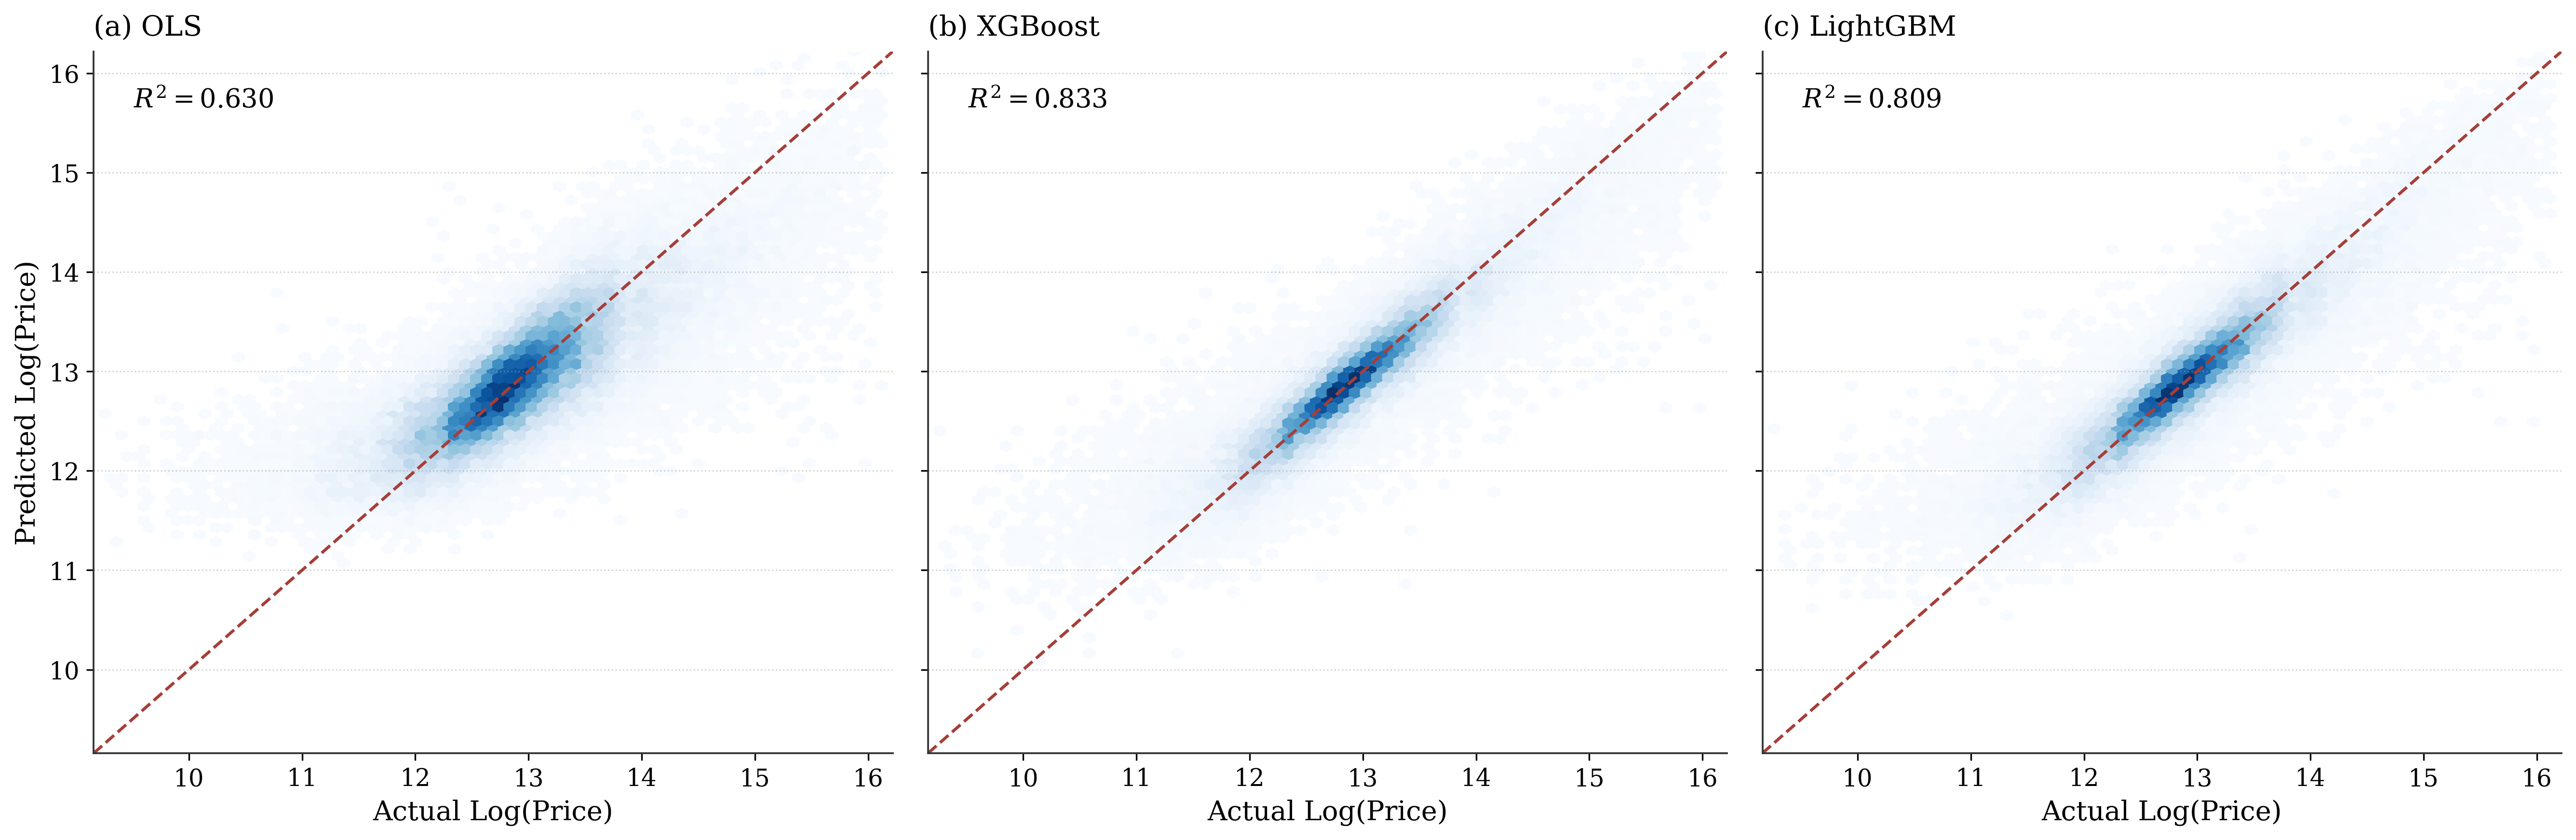
\includegraphics[width=\textwidth]{figures/fig4_model_comparison.png}
    \caption{Predicted vs.\ Actual Log-Prices Under Random Validation: (a) OLS; (b) XGBoost; (c) LightGBM}
    \label{fig:model_comparison}
\end{figure}


\subsection{Machine Learning Under Geographic Validation}
\label{sec:ml_geo}

Table~\ref{tab:geo_holdout} reports performance when 10 states are held out entirely.

\begin{table}[H]
\centering
\caption{Geographic Holdout Validation (10 States Held Out)}
\label{tab:geo_holdout}
\begin{threeparttable}
\begin{tabular}{lrrr}
\toprule
Model & $R^2$ (random) & $R^2$ (geo holdout) & $\Delta R^2$ \\
\midrule
OLS & 0.630 & $<0$ & $>-0.63$ \\
Random Forest & 0.784 & 0.542 & $-0.242$ \\
XGBoost & 0.833 & 0.547 & $-0.286$ \\
XGBoost (no geo features) & 0.830 & 0.519 & $-0.311$ \\
XGBoost (+ lat/lon) & 0.870 & 0.464 & $-0.406$ \\
\bottomrule
\end{tabular}
\begin{tablenotes}
\small
\item \textit{Notes:} Geographic holdout: CA, NY, TX, FL, OH, CO, NC, WA, IL, GA held out (438,315 observations). Training on remaining 350,527 observations. OLS with regional dummies fails catastrophically because the held-out states span all four Census regions and include the largest markets. ``No geo features'' removes region dummies from the full model. ``+ lat/lon'' adds raw latitude and longitude as continuous features.
\end{tablenotes}
\end{threeparttable}
\end{table}

\textbf{Key finding.} The XGBoost $R^2$ drops from 0.833 (random) to 0.547 (geographic holdout)---a \textbf{28.6-percentage-point decline}. This demonstrates that a substantial portion of the random-validation $R^2$ reflects the model's ability to exploit local spatial structure rather than learning generalizable attribute-price relationships.

Two additional experiments sharpen this conclusion:
\begin{itemize}[nosep]
    \item \textbf{Adding latitude and longitude} boosts random $R^2$ from 0.833 to 0.870 ($+3.7$ pp) but \emph{reduces} geographic holdout $R^2$ to 0.464 ($-8.3$ pp relative to the baseline XGBoost). Coordinates allow the model to memorize location-specific price levels, which is useful when nearby properties appear in the test set but harmful when entire states are withheld.
    \item \textbf{Removing all geographic features} (no region dummies) yields random $R^2 = 0.830$ (essentially unchanged) but geographic holdout $R^2 = 0.519$. Compared to the ablation-design variant of the full model (Geo $R^2 = 0.425$; see Section~\ref{sec:ablation}), dropping geography \emph{improves} geographic holdout by $+9.4$ pp. Region dummies can \emph{harm} geographic generalization because they encode training-set-specific geographic price levels.
\end{itemize}

This finding is methodologically important: \textbf{random train-test splits can substantially overstate the predictive performance of hedonic models} when applied to geographically diverse national samples. Geographic holdout validation provides a more conservative---and arguably more relevant---assessment of model generalizability.


\subsection{Ablation: What Drives the ML Gain?}
\label{sec:ablation}

Table~\ref{tab:ablation} presents the results of the feature ablation analysis for XGBoost.

\begin{table}[H]
\centering
\caption{XGBoost Ablation Analysis: Marginal Contribution of Feature Groups}
\label{tab:ablation}
\begin{threeparttable}
\small
\begin{tabular}{llrrrr}
\toprule
Stage & Feature Set & $N_{\text{features}}$ & Random $R^2$ & Geo $R^2$ & $\Delta$ Geo $R^2$ \\
\midrule
1 & Structural only & 8 & 0.4976 & 0.3481 & --- \\
2 & + Lot & 9 & 0.5464 & 0.3765 & $+$0.028 \\
3 & + Amenities & 20 & 0.6378 & 0.4485 & $+$0.072 \\
4 & + Neighborhood & 27 & 0.8136 & 0.4833 & $+$0.035 \\
5 & + Market status & 32 & 0.8235 & 0.5014 & $+$0.018 \\
6 & Full model (+ interactions/cats/region) & 62 & 0.8327 & 0.4250 & $-$0.076 \\
\bottomrule
\end{tabular}
\begin{tablenotes}
\small
\item \textit{Notes:} Each row adds a feature group to the previous stage. Random $R^2$ is computed on the standard 20\% random holdout. Geo $R^2$ is computed on the 10-state geographic holdout. $\Delta$ Geo $R^2$ is the change from the previous stage.
\end{tablenotes}
\end{threeparttable}
\end{table}

Three findings emerge from the ablation analysis.

\textbf{Neighborhood features provide the largest random-validation gain.} Adding neighborhood variables (Walk Score, Bike Score, Transit Score, school rating, school count, school distance, tax rate) increases random $R^2$ from 0.638 to 0.814---a gain of $+17.6$ pp. This is more than twice the contribution of any other feature group, reflecting the importance of local amenities and public-service quality in explaining listing-price variation.

\textbf{The full model hurts geographic generalization.} The transition from Stage 5 (32 features, Geo $R^2 = 0.501$) to Stage 6 (62 features, Geo $R^2 = 0.425$) \emph{reduces} geographic holdout $R^2$ by 7.6 pp. The features added in Stage 6 include region dummies, interaction terms involving region, and categorical controls. These features improve random $R^2$ modestly ($+0.9$ pp) but actively harm geographic generalization by encoding training-set-specific spatial patterns.

\textbf{Structural features alone explain 35\% of geographic variation.} Even with only 8 structural variables, XGBoost achieves Geo $R^2 = 0.348$, indicating that basic property characteristics (size, bedrooms, bathrooms, age) carry non-trivial predictive power across geographies.


\subsection{The Role of Geographic Features}
\label{sec:geo_features}

The ablation and geographic holdout results jointly demonstrate a critical tension in hedonic modeling: geographic features improve in-sample and random-holdout fit but degrade geographic generalization. Table~\ref{tab:geo_role} summarizes the evidence.

\begin{table}[H]
\centering
\caption{Impact of Geographic Features on Model Performance}
\label{tab:geo_role}
\begin{threeparttable}
\small
\begin{tabular}{lrr}
\toprule
XGBoost Specification & Random $R^2$ & Geographic Holdout $R^2$ \\
\midrule
Full model (62 features, with region) & 0.8327 & 0.4250 \\
No geographic features (no region dummies) & 0.8297 & 0.5190 \\
Full model + lat/lon coordinates & 0.8701 & 0.4644 \\
\bottomrule
\end{tabular}
\begin{tablenotes}
\small
\item \textit{Notes:} ``No geographic features'' removes region dummies from the full model. ``+ lat/lon'' adds raw latitude and longitude as continuous features to the full model. Geographic holdout uses 10 states held out entirely.
\end{tablenotes}
\end{threeparttable}
\end{table}

Removing region dummies costs only 0.3 pp in random $R^2$ (0.833 to 0.830) but \emph{gains} 9.4 pp in geographic holdout $R^2$ (0.425 to 0.519). Adding coordinates achieves the opposite: $+3.7$ pp random, $-5.5$ pp geographic holdout (relative to the no-geography specification).

This pattern has important implications for automated valuation models (AVMs). In deployment contexts where the model must generalize to new geographies, geographic features can be counterproductive. The model without geography exploits only attribute-price relationships that transfer across markets, yielding more conservative but more robust predictions.


\subsection{SHAP Analysis and Cross-Model Stability}
\label{sec:shap_results}

\subsubsection{Feature Importance Rankings}

Table~\ref{tab:shap_importance} reports the top 20 features by mean absolute SHAP value from the XGBoost model.

\begin{table}[H]
\centering
\caption{Top 20 Features by Mean Absolute SHAP Value (XGBoost)}
\label{tab:shap_importance}
\begin{threeparttable}
\begin{tabular}{rlr}
\toprule
Rank & Feature & Mean $|\phi|$ \\
\midrule
1 & $\ln$(Living Area) & 0.1740 \\
2 & Bathrooms & 0.1610 \\
3 & Avg.\ School Rating & 0.0881 \\
4 & Region: West & 0.0751 \\
5 & $\ln$(Lot Size) & 0.0747 \\
6 & Luxury Score & 0.0713 \\
7 & Property Tax Rate & 0.0694 \\
8 & Nearest School Distance & 0.0472 \\
9 & Region: Northeast & 0.0425 \\
10 & Bike Score & 0.0400 \\
11 & $\ln$(HOA Fees + 1) & 0.0398 \\
12 & Garage & 0.0378 \\
13 & Age & 0.0369 \\
14 & Hardwood Floors & 0.0311 \\
15 & Waterfront $\times$ $\ln$(sqft) & 0.0292 \\
16 & Sqft per Bedroom & 0.0289 \\
17 & Walk Score & 0.0276 \\
18 & Central Air & 0.0273 \\
19 & Region: South & 0.0250 \\
20 & Transit Score & 0.0213 \\
\bottomrule
\end{tabular}
\begin{tablenotes}
\small
\item \textit{Notes:} TreeSHAP values computed on 10,000 random test-set observations. Mean $|\phi|$ is the average absolute contribution of each feature to deviations from the expected predicted log-price. These are predictive contributions, not structural implicit prices.
\end{tablenotes}
\end{threeparttable}
\end{table}

\begin{figure}[H]
    \centering
    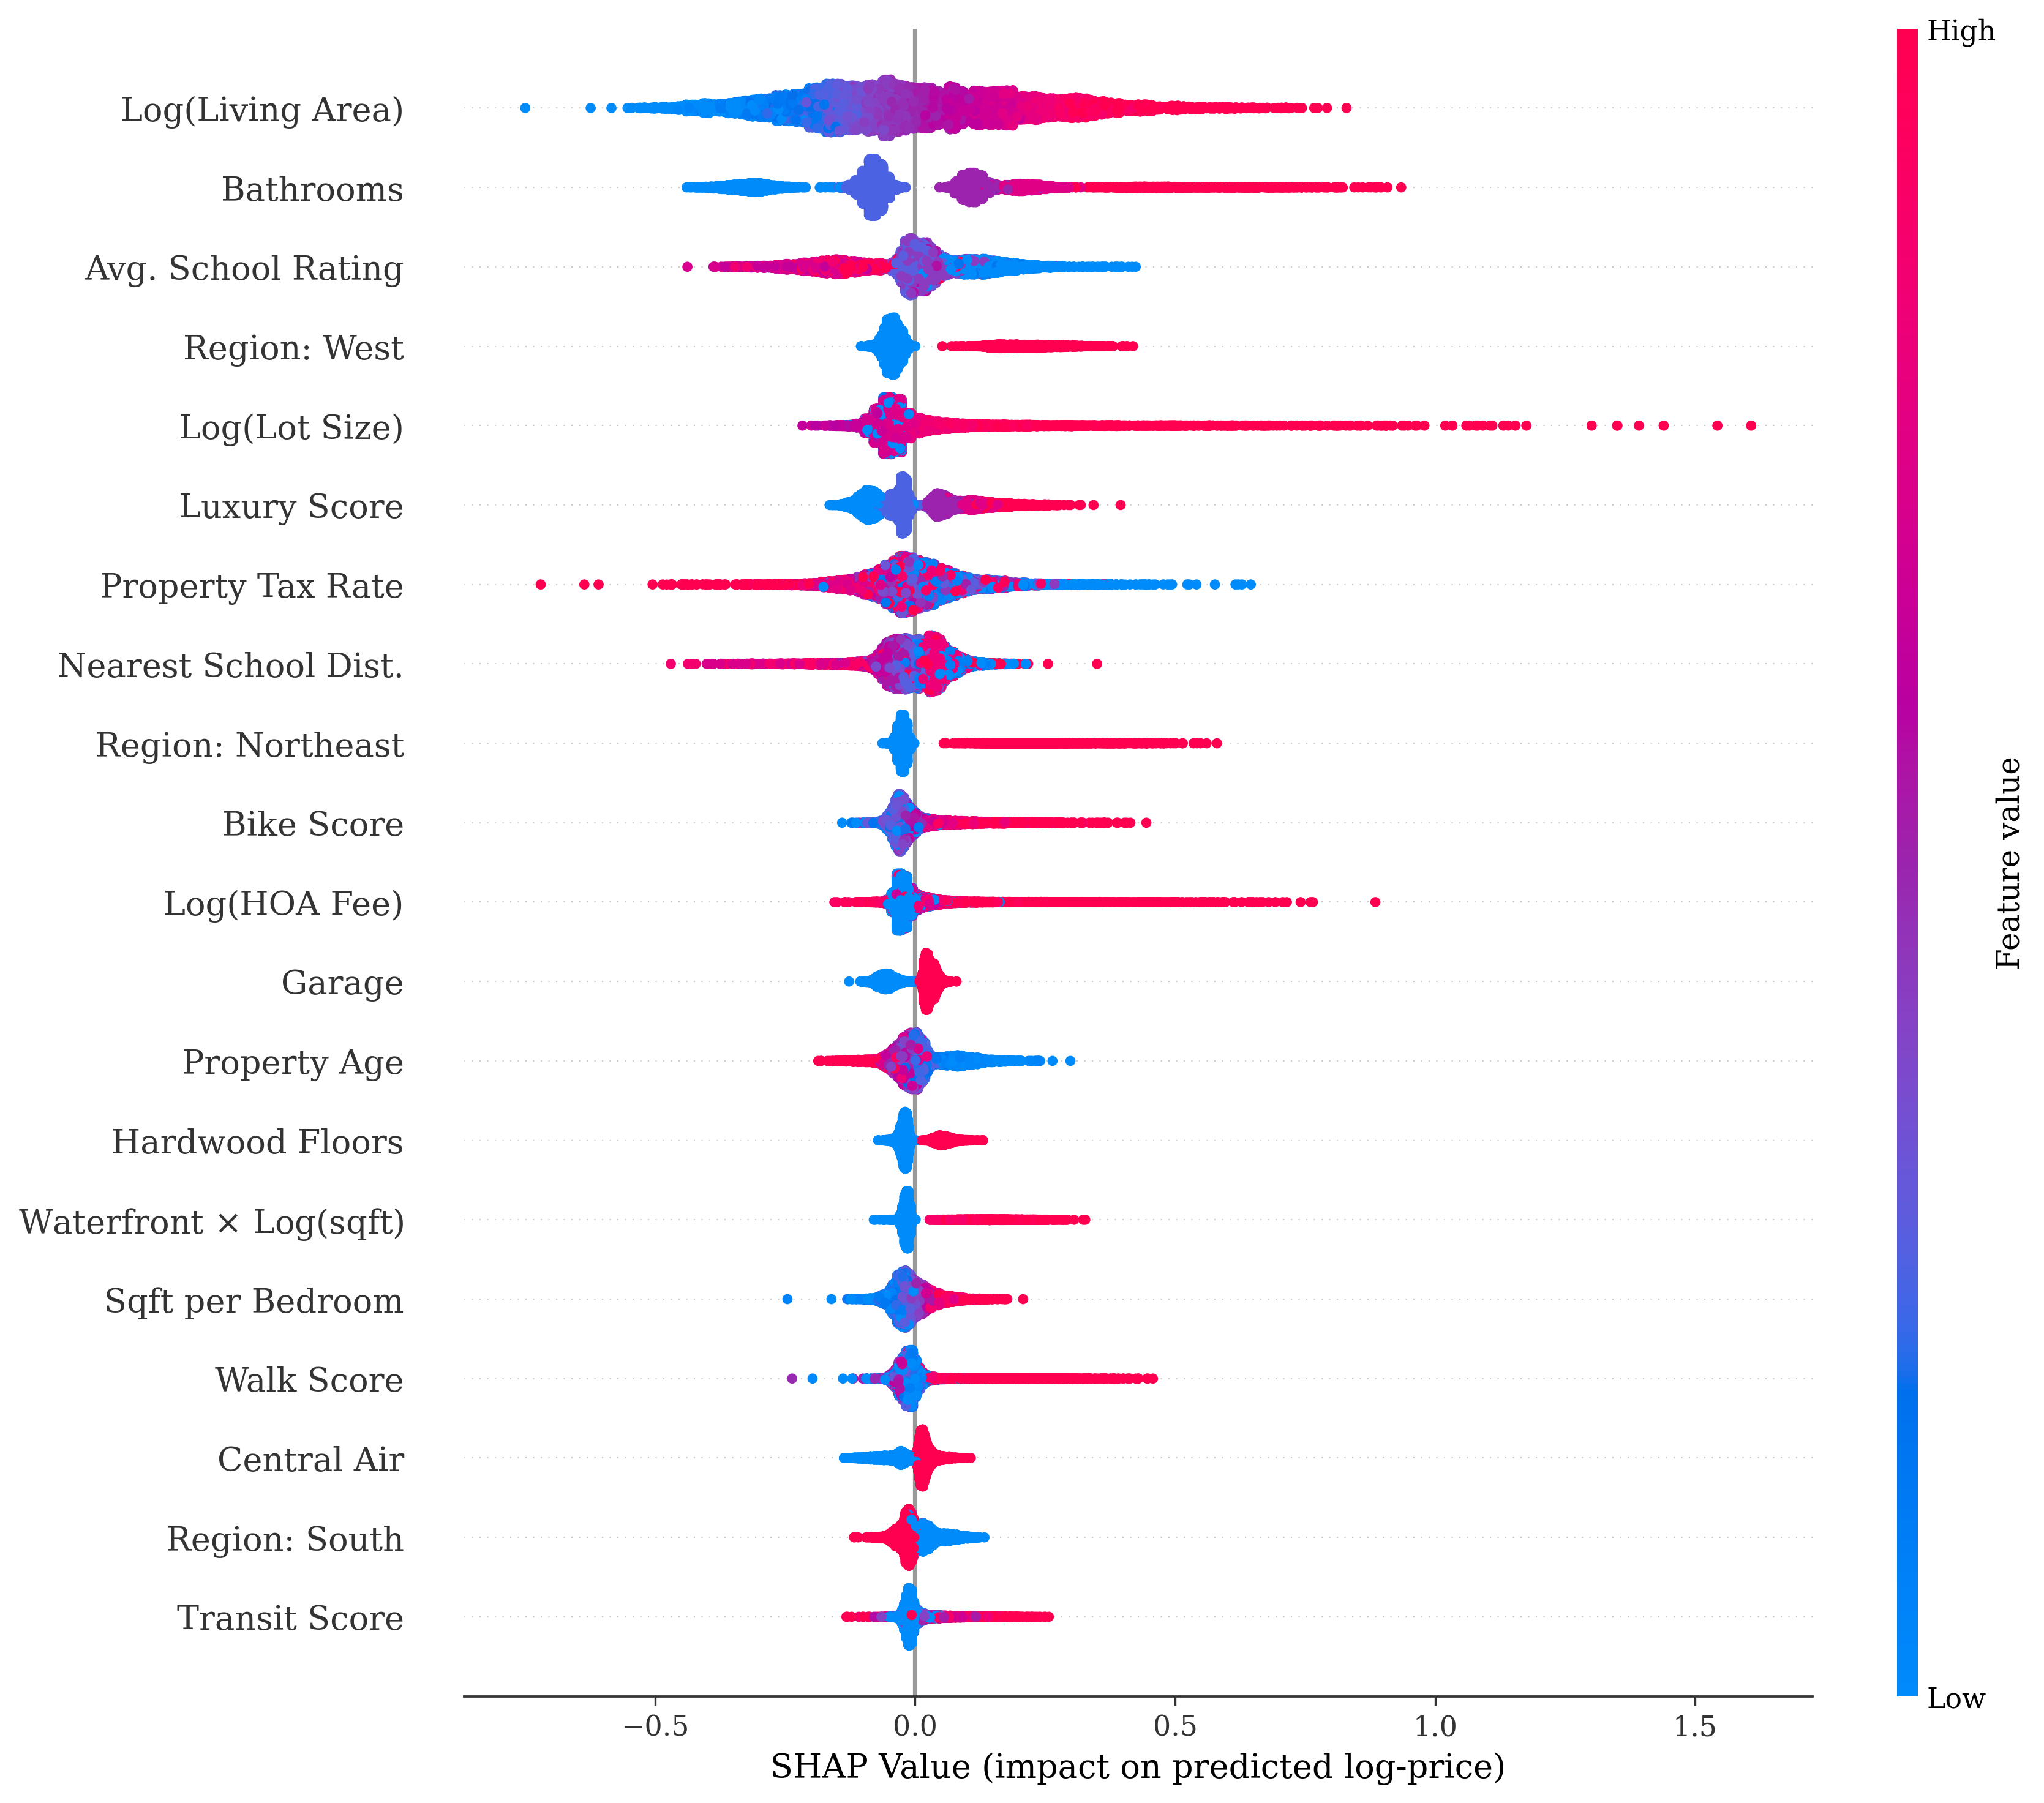
\includegraphics[width=0.85\textwidth]{figures/fig5_shap_summary.png}
    \caption{SHAP Summary Plot for XGBoost. Each dot is one observation; horizontal position shows the feature's SHAP value (contribution to predicted log-price deviation from the mean); color indicates feature value (red = high, blue = low). These are predictive contributions, not causal effects.}
    \label{fig:shap_summary}
\end{figure}

Living area and bathrooms are the two dominant predictive contributors, with mean absolute SHAP values of 0.174 and 0.161. School quality (0.088), regional location (West: 0.075; Northeast: 0.043), and lot size (0.075) form a second tier.

\textbf{SHAP dependence plots.} Figure~\ref{fig:shap_dependence} shows how the SHAP contribution of key features varies with feature values. The non-linear shapes---particularly the strongly concave living-area SHAP and the threshold-like behavior of school rating and property tax rate---explain why tree-based models outperform linear OLS. These non-linearities cannot be captured by the semi-log specification even with interaction terms.

\begin{figure}[H]
    \centering
    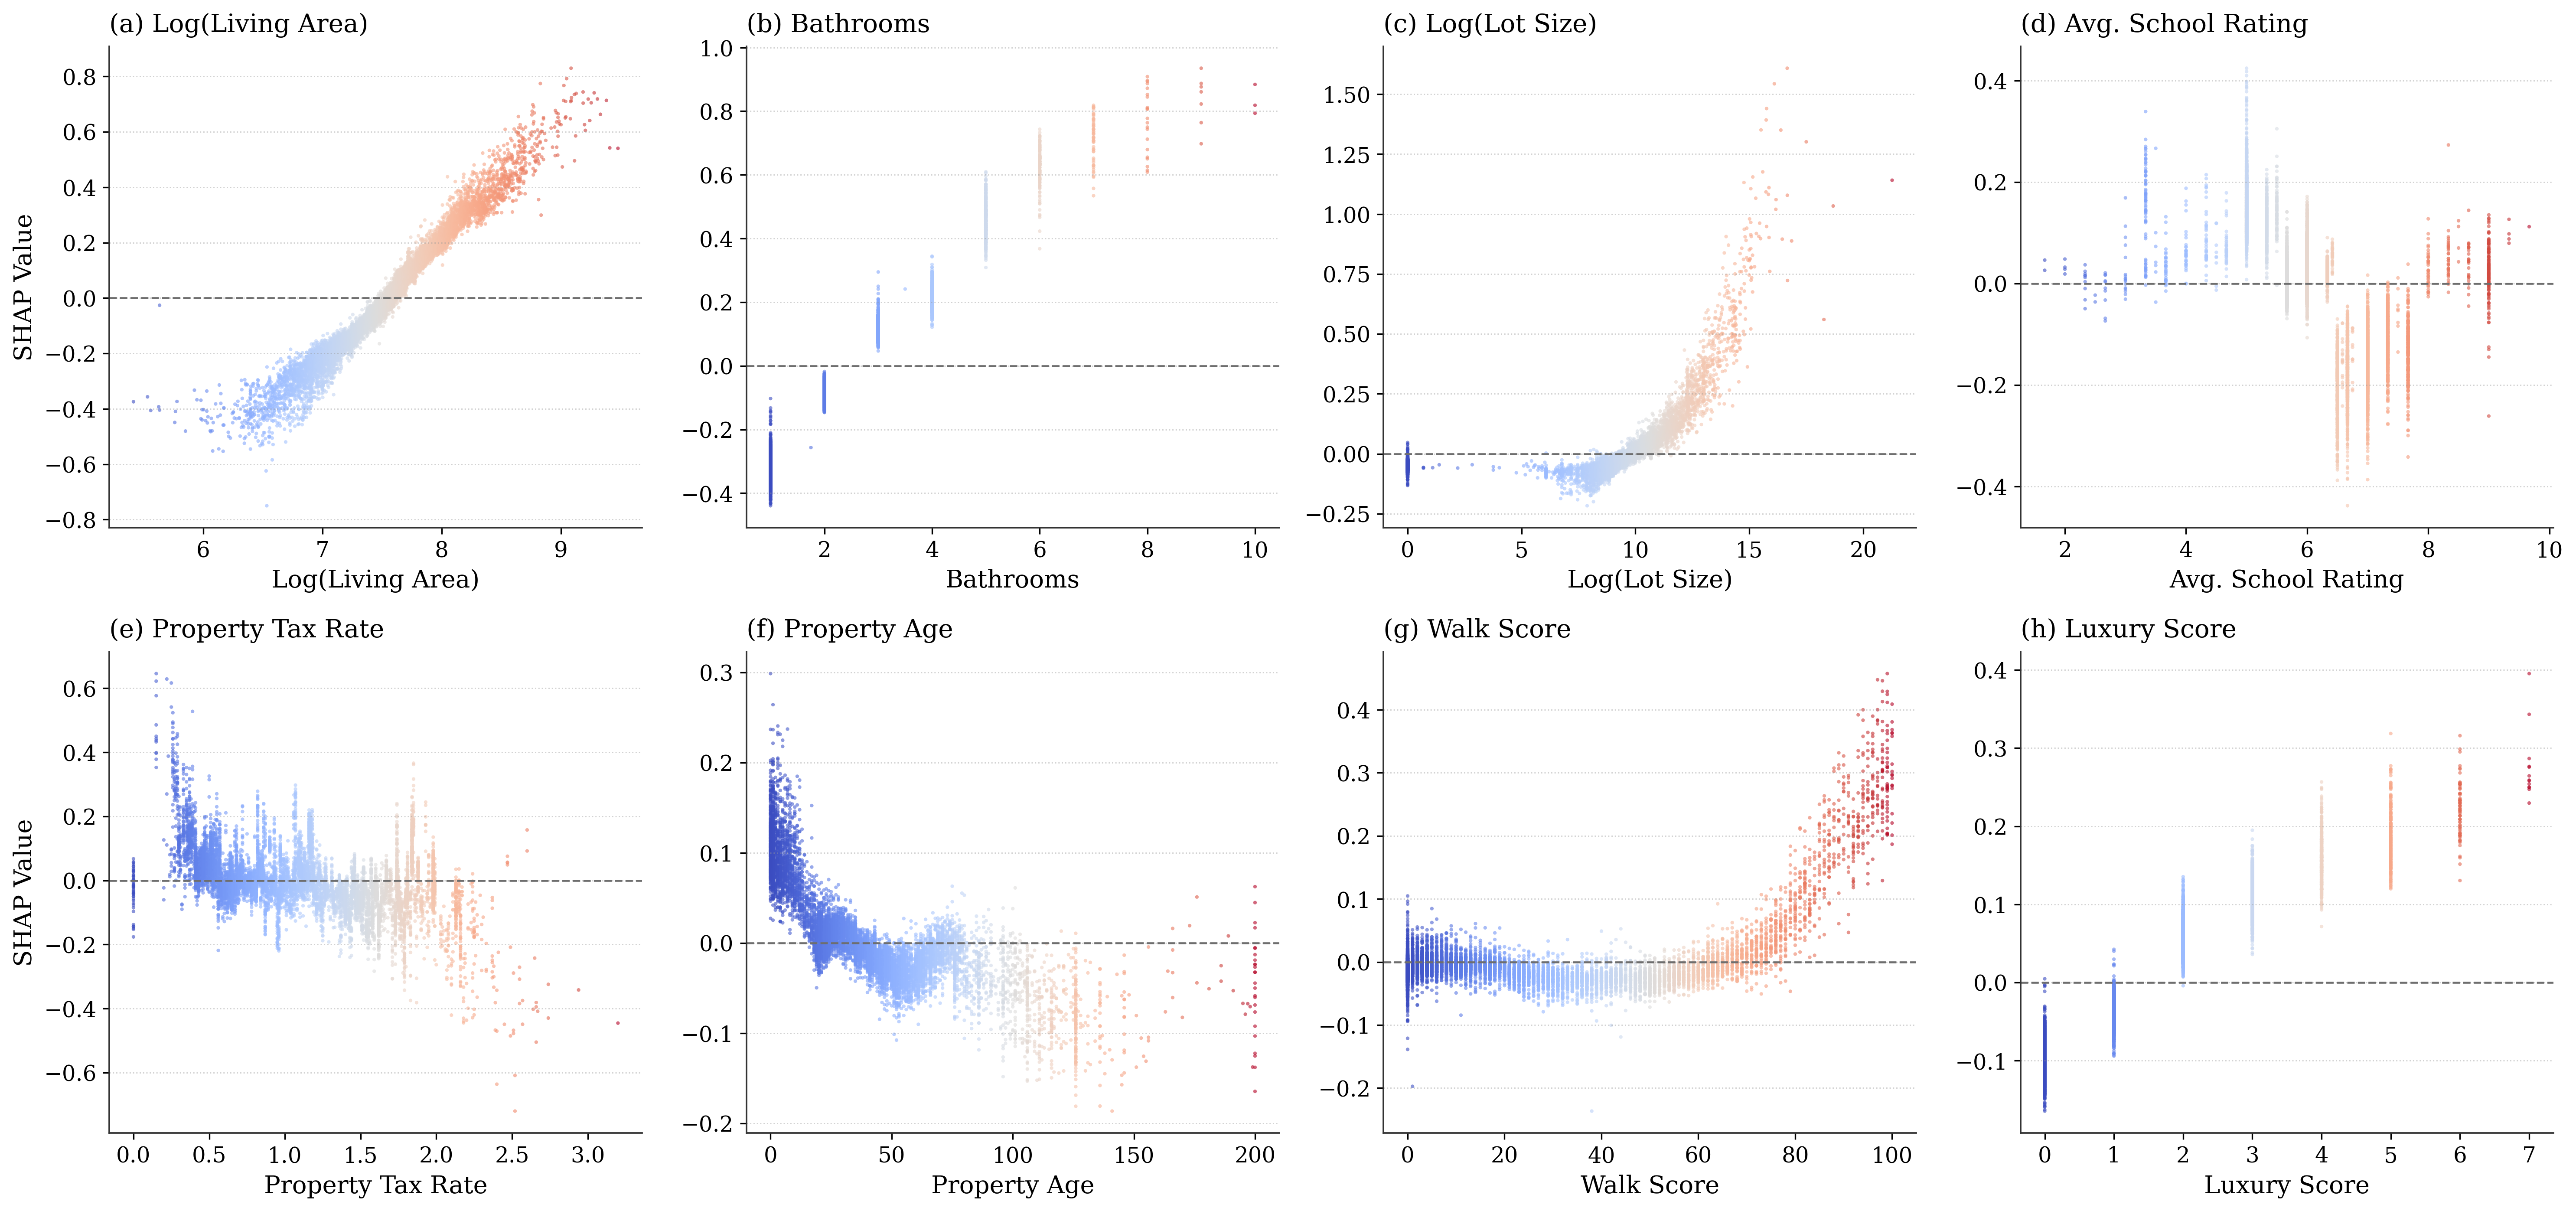
\includegraphics[width=\textwidth]{figures/fig10_shap_dependence.png}
    \caption{SHAP Dependence Plots for Eight Key Features. Each panel shows how the SHAP contribution varies with the feature value. Non-linear patterns (concavity, thresholds, saturation) explain the predictive advantage of tree-based models over linear specifications.}
    \label{fig:shap_dependence}
\end{figure}

\subsubsection{Cross-Model SHAP Stability}

A common concern with SHAP-based interpretation is that rankings may be model-specific artifacts. Table~\ref{tab:shap_stability} reports pairwise Spearman rank correlations of mean absolute SHAP values across three tree-based models.

\begin{table}[H]
\centering
\caption{Cross-Model SHAP Importance Stability: Spearman Rank Correlations}
\label{tab:shap_stability}
\begin{threeparttable}
\begin{tabular}{lrrr}
\toprule
& XGBoost & LightGBM & Random Forest \\
\midrule
XGBoost & 1.000 & 0.9898 & 0.9060 \\
LightGBM & 0.9898 & 1.000 & 0.8917 \\
Random Forest & 0.9060 & 0.8917 & 1.000 \\
\bottomrule
\end{tabular}
\begin{tablenotes}
\small
\item \textit{Notes:} Spearman $\rho$ computed on the full vector of mean $|\phi|$ values across all features. The same six features---$\ln$(Living Area), Bathrooms, Avg.\ School Rating, Region: West, $\ln$(Lot Size), and Luxury Score---rank in the top six across all three models.
\end{tablenotes}
\end{threeparttable}
\end{table}

The cross-model correlations are remarkably high. XGBoost and LightGBM produce nearly identical rankings ($\rho = 0.990$), while even the structurally different Random Forest model yields $\rho > 0.89$ with both gradient-boosted methods. The same six features appear in the top six across all three models. This stability lends credibility to the SHAP-based feature importance ranking as a description of the predictive structure of the data, not merely an artifact of a particular algorithm.

\textbf{Note on SHAP versus OLS comparisons.} SHAP importance rankings differ from both OLS $t$-statistics and XGBoost gain importance. School rating ranks 3rd by SHAP but has a counterintuitive negative OLS sign; property tax rate ranks 7th by SHAP but 28th by standardized OLS coefficient magnitude. These discrepancies reflect the non-linear and interactive effects that SHAP captures but OLS cannot. However, even though SHAP rankings are stable across tree-based models, they should not be interpreted as revealing the ``true'' importance hierarchy of housing attributes---they remain predictive decompositions, not structural parameters.


\subsection{Geographic Heterogeneity}

Figure~\ref{fig:geographic} maps the spatial distribution of listing prices. The well-documented coastal price gradient is clearly visible, with California, the Northeast corridor, Hawaii, and Colorado exhibiting the highest prices. The map also illustrates the non-representativeness concern: listing density is highly uneven, with sparse coverage in some rural areas.

\begin{figure}[H]
    \centering
    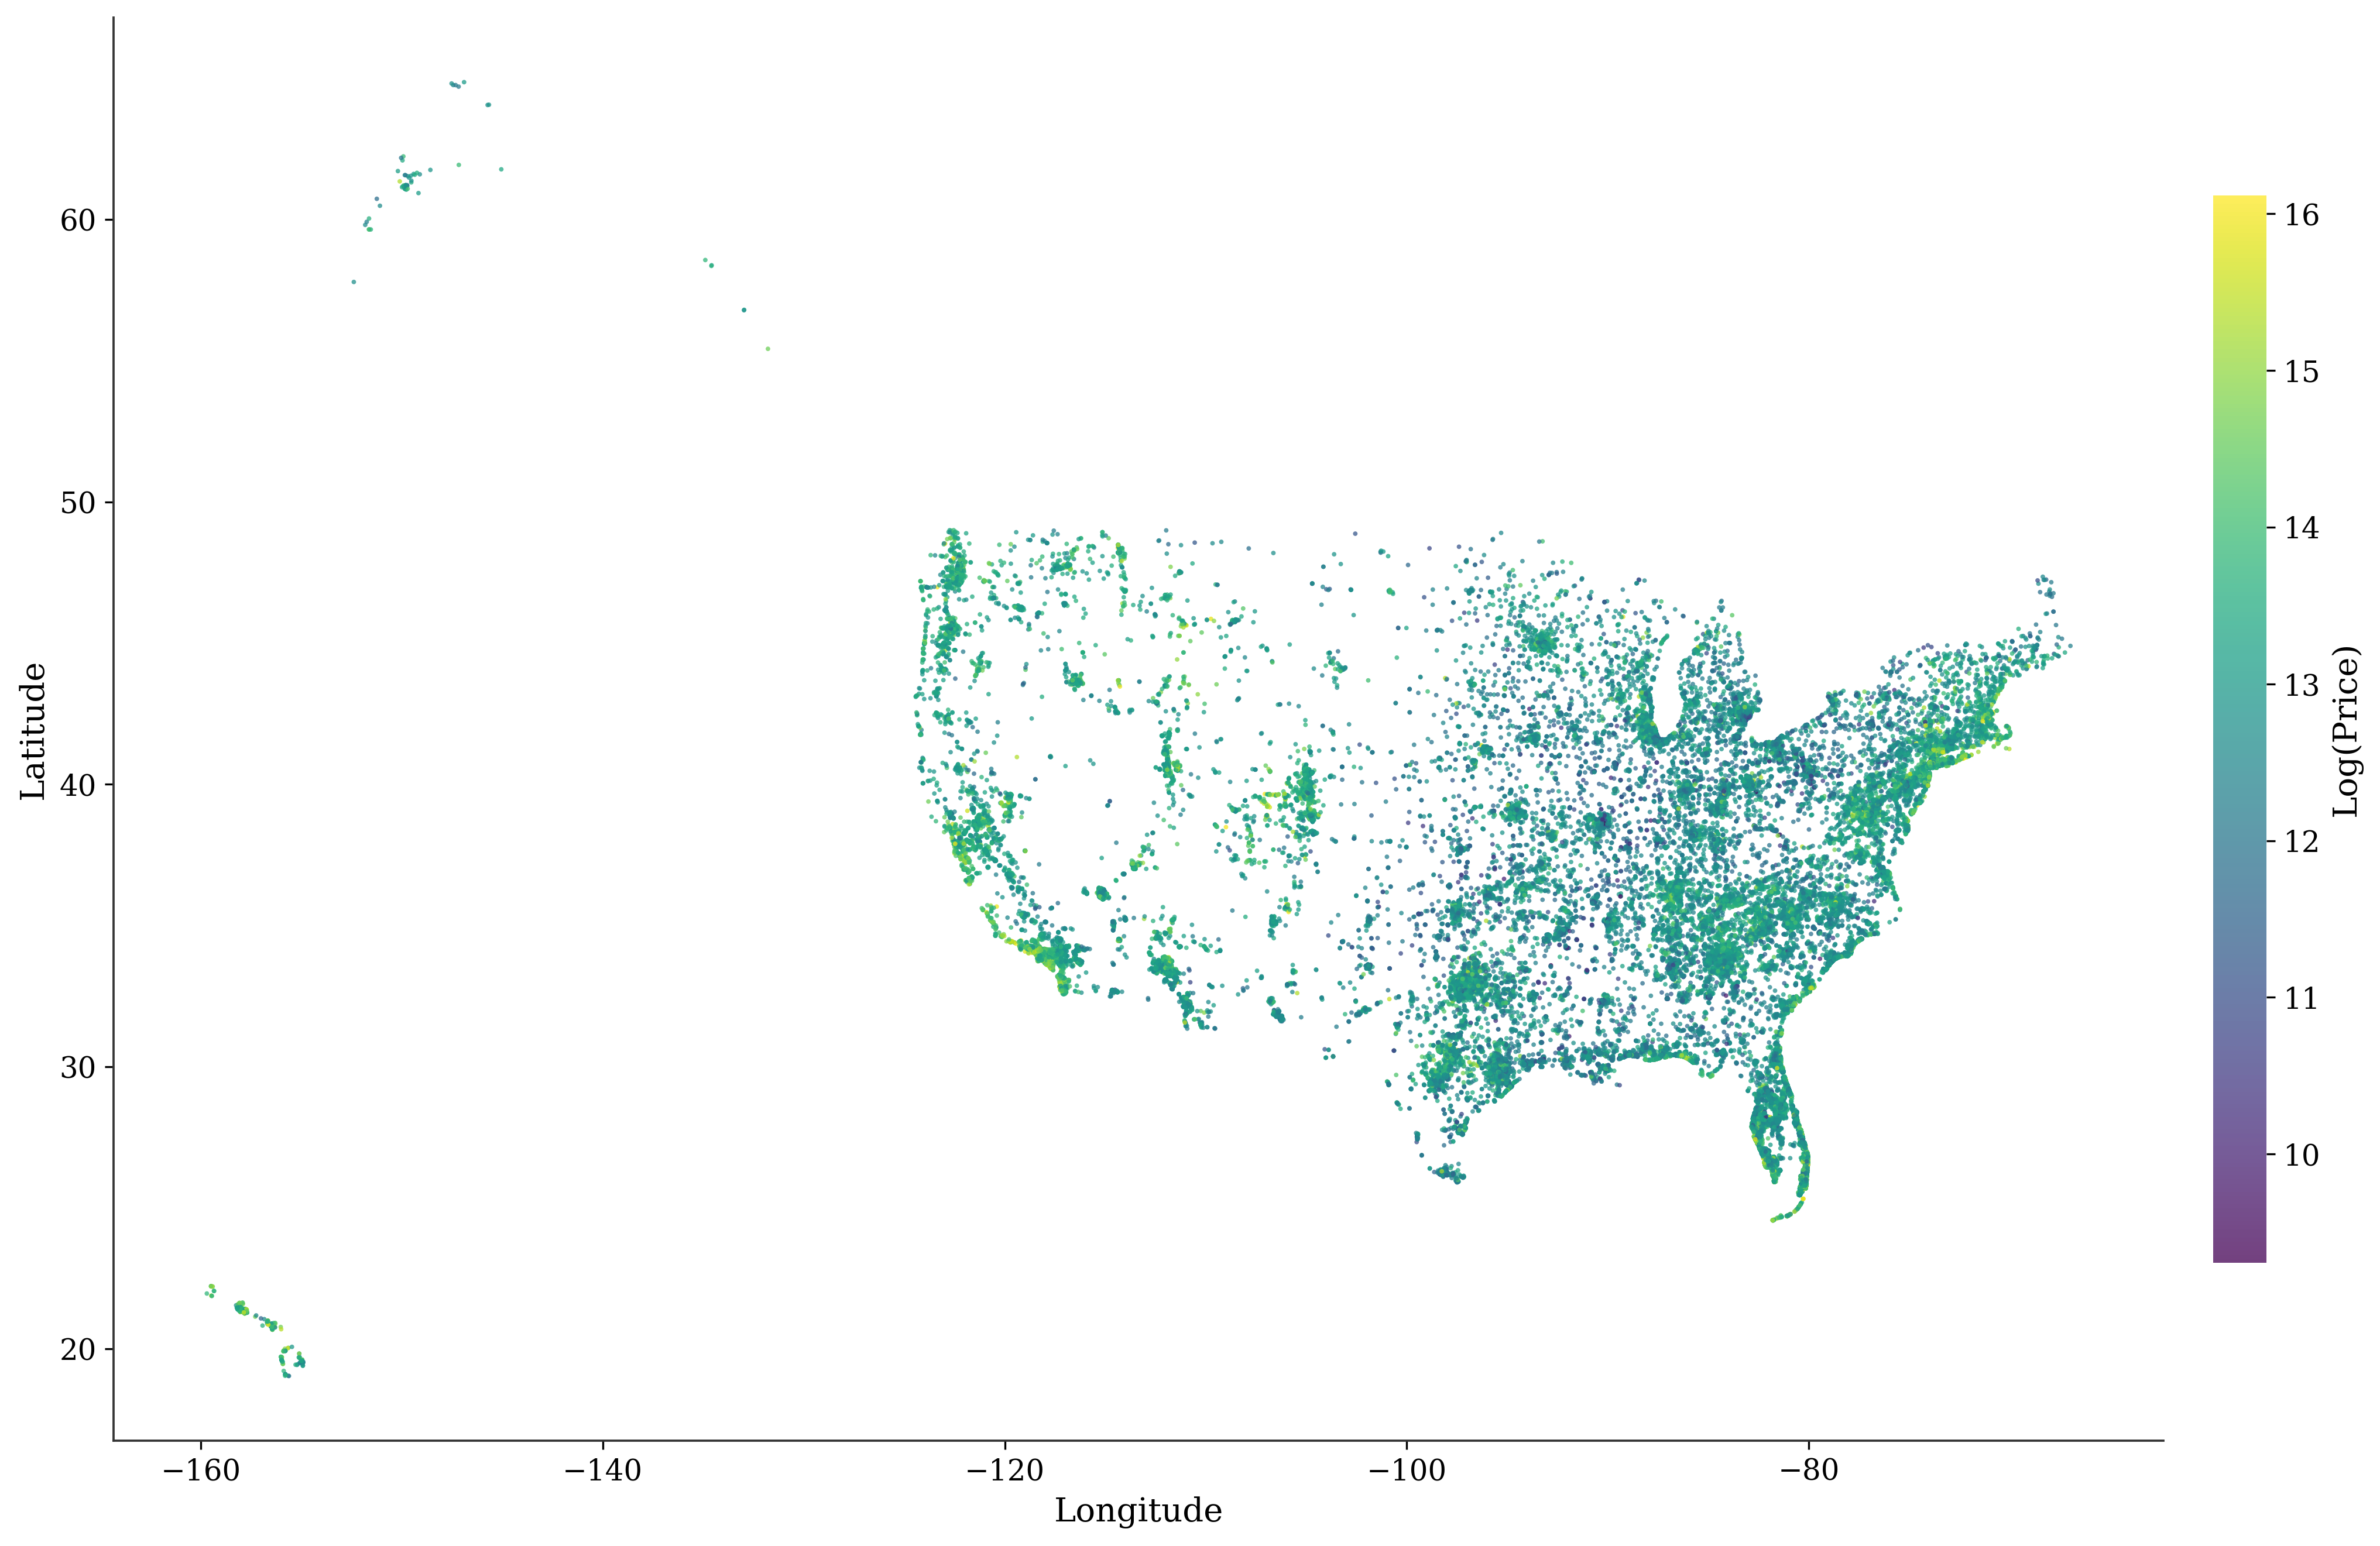
\includegraphics[width=\textwidth]{figures/fig7_geographic_prices.png}
    \caption{Geographic Distribution of Log Listing Prices. Each dot represents one property (50,000 random subsample). Color indicates log-price. Note: listing density is not uniform; areas with few dots may have fewer Zillow listings, not necessarily fewer properties.}
    \label{fig:geographic}
\end{figure}

\begin{figure}[H]
    \centering
    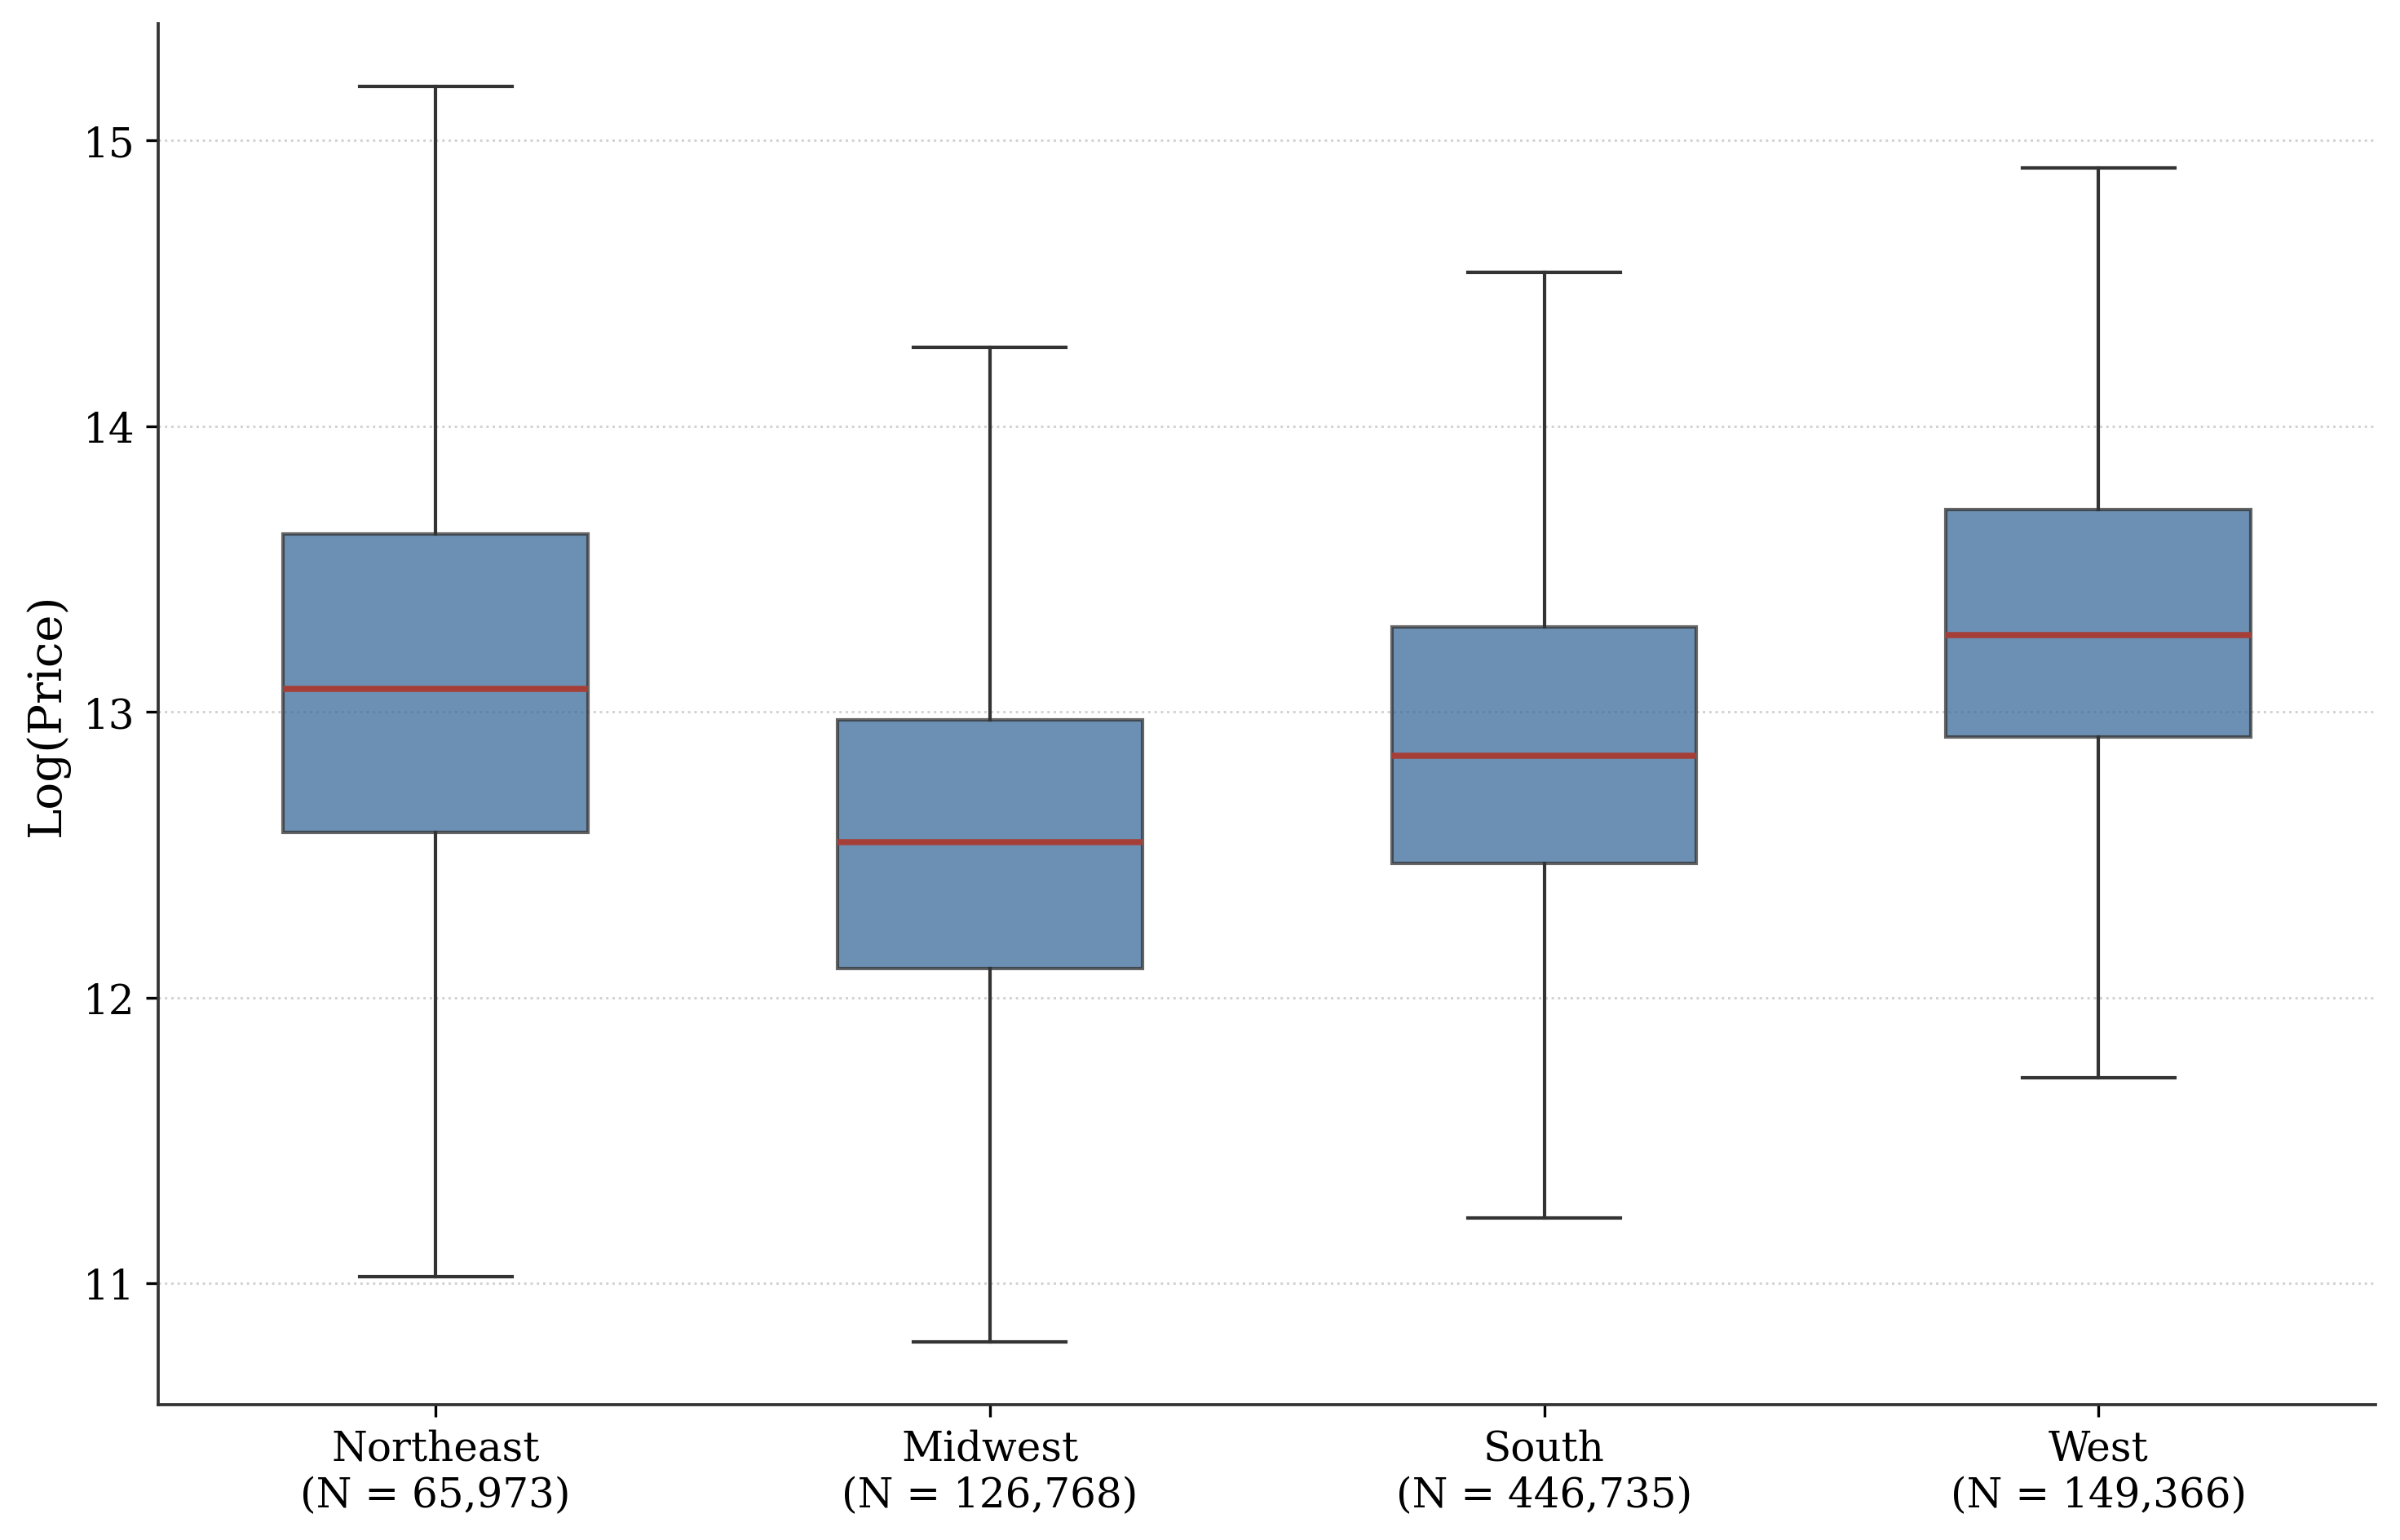
\includegraphics[width=0.85\textwidth]{figures/fig8_regional_prices.png}
    \caption{Listing Price Distribution by Census Region}
    \label{fig:regional}
\end{figure}


\subsection{Non-Linear Relationships}

Figure~\ref{fig:marginal} presents bivariate (unconditional) relationships between key attributes and log listing prices. These plots illustrate the non-linearities that motivate the machine learning approach but should not be confused with conditional (ceteris paribus) effects.

\begin{figure}[H]
    \centering
    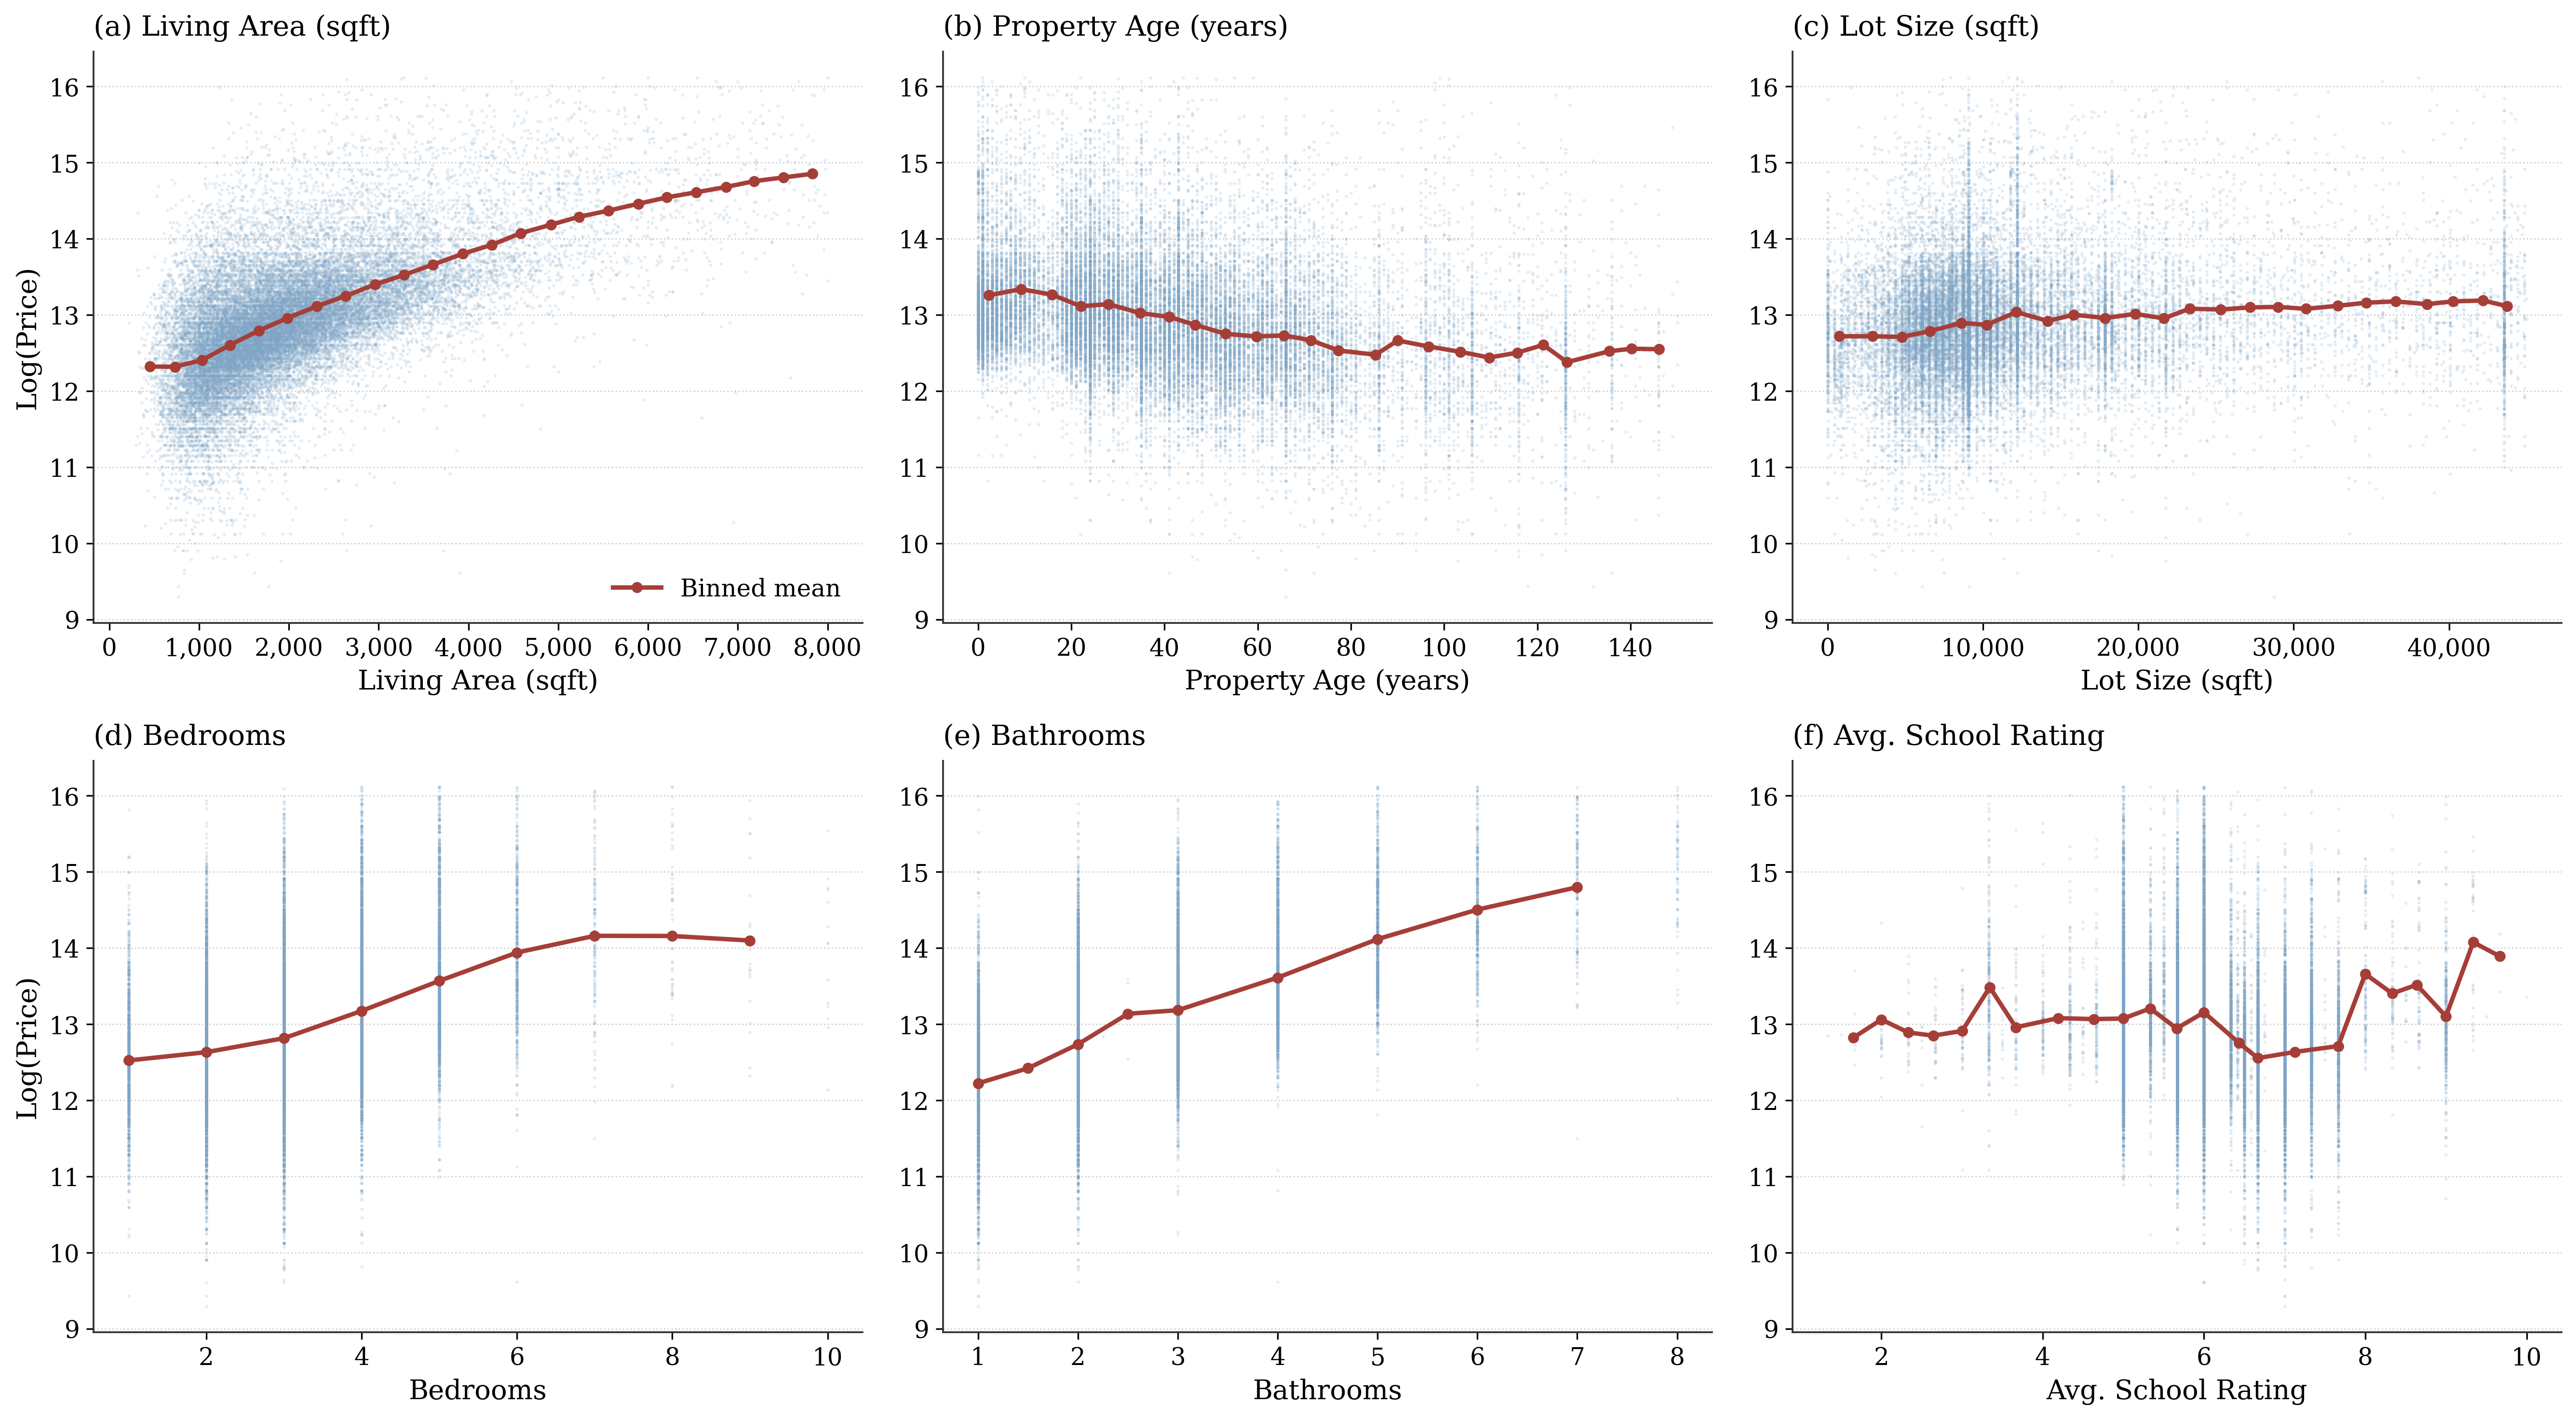
\includegraphics[width=\textwidth]{figures/fig9_marginal_effects.png}
    \caption{Unconditional Bivariate Relationships Between Key Attributes and Log Listing Price. These are raw scatter plots and binned means; they do not control for other attributes and should not be interpreted as conditional effects.}
    \label{fig:marginal}
\end{figure}
